\documentclass[twoside]{book}

% Packages required by doxygen
\usepackage{fixltx2e}
\usepackage{calc}
\usepackage{doxygen}
\usepackage[export]{adjustbox} % also loads graphicx
\usepackage{graphicx}
\usepackage[utf8]{inputenc}
\usepackage{makeidx}
\usepackage{multicol}
\usepackage{multirow}
\PassOptionsToPackage{warn}{textcomp}
\usepackage{textcomp}
\usepackage[nointegrals]{wasysym}
\usepackage[table]{xcolor}

% Font selection
\usepackage[T1]{fontenc}
\usepackage[scaled=.90]{helvet}
\usepackage{courier}
\usepackage{amssymb}
\usepackage{sectsty}
\renewcommand{\familydefault}{\sfdefault}
\allsectionsfont{%
  \fontseries{bc}\selectfont%
  \color{darkgray}%
}
\renewcommand{\DoxyLabelFont}{%
  \fontseries{bc}\selectfont%
  \color{darkgray}%
}
\newcommand{\+}{\discretionary{\mbox{\scriptsize$\hookleftarrow$}}{}{}}

% Page & text layout
\usepackage{geometry}
\geometry{%
  a4paper,%
  top=2.5cm,%
  bottom=2.5cm,%
  left=2.5cm,%
  right=2.5cm%
}
\tolerance=750
\hfuzz=15pt
\hbadness=750
\setlength{\emergencystretch}{15pt}
\setlength{\parindent}{0cm}
\setlength{\parskip}{0.2cm}
\makeatletter
\renewcommand{\paragraph}{%
  \@startsection{paragraph}{4}{0ex}{-1.0ex}{1.0ex}{%
    \normalfont\normalsize\bfseries\SS@parafont%
  }%
}
\renewcommand{\subparagraph}{%
  \@startsection{subparagraph}{5}{0ex}{-1.0ex}{1.0ex}{%
    \normalfont\normalsize\bfseries\SS@subparafont%
  }%
}
\makeatother

% Headers & footers
\usepackage{fancyhdr}
\pagestyle{fancyplain}
\fancyhead[LE]{\fancyplain{}{\bfseries\thepage}}
\fancyhead[CE]{\fancyplain{}{}}
\fancyhead[RE]{\fancyplain{}{\bfseries\leftmark}}
\fancyhead[LO]{\fancyplain{}{\bfseries\rightmark}}
\fancyhead[CO]{\fancyplain{}{}}
\fancyhead[RO]{\fancyplain{}{\bfseries\thepage}}
\fancyfoot[LE]{\fancyplain{}{}}
\fancyfoot[CE]{\fancyplain{}{}}
\fancyfoot[RE]{\fancyplain{}{\bfseries\scriptsize Generated on Sat Nov 21 2015 11\+:55\+:49 for Bowling 3\+D by Doxygen }}
\fancyfoot[LO]{\fancyplain{}{\bfseries\scriptsize Generated on Sat Nov 21 2015 11\+:55\+:49 for Bowling 3\+D by Doxygen }}
\fancyfoot[CO]{\fancyplain{}{}}
\fancyfoot[RO]{\fancyplain{}{}}
\renewcommand{\footrulewidth}{0.4pt}
\renewcommand{\chaptermark}[1]{%
  \markboth{#1}{}%
}
\renewcommand{\sectionmark}[1]{%
  \markright{\thesection\ #1}%
}

% Indices & bibliography
\usepackage{natbib}
\usepackage[titles]{tocloft}
\setcounter{tocdepth}{3}
\setcounter{secnumdepth}{5}
\makeindex

% Hyperlinks (required, but should be loaded last)
\usepackage{ifpdf}
\ifpdf
  \usepackage[pdftex,pagebackref=true]{hyperref}
\else
  \usepackage[ps2pdf,pagebackref=true]{hyperref}
\fi
\hypersetup{%
  colorlinks=true,%
  linkcolor=blue,%
  citecolor=blue,%
  unicode%
}

% Custom commands
\newcommand{\clearemptydoublepage}{%
  \newpage{\pagestyle{empty}\cleardoublepage}%
}


%===== C O N T E N T S =====

\begin{document}

% Titlepage & ToC
\hypersetup{pageanchor=false,
             bookmarks=true,
             bookmarksnumbered=true,
             pdfencoding=unicode
            }
\pagenumbering{roman}
\begin{titlepage}
\vspace*{7cm}
\begin{center}%
{\Large Bowling 3\+D }\\
\vspace*{1cm}
{\large Generated by Doxygen 1.8.10}\\
\vspace*{0.5cm}
{\small Sat Nov 21 2015 11:55:49}\\
\end{center}
\end{titlepage}
\clearemptydoublepage
\tableofcontents
\clearemptydoublepage
\pagenumbering{arabic}
\hypersetup{pageanchor=true}

%--- Begin generated contents ---
\chapter{Pins movement}
\label{_pins_01movement}
\hypertarget{_pins_01movement}{}
This document describes the way the bowling pins are moving.

Zaimplementowano kilka rodzajów ruchu kręgli. Jednym z nich jest ruch po kwadracie w płaszczyźnie poziomej. Występuje także ruch po okręgu w płaszczyźnie pionowej, a także ruch po okręgu, gdzie prędkość jest zmienna i jest funkcją czasu. Dodano także symulację eksplozji poprzez przyłożenie siły do bryły sztywnej. Dwa najbardziej skrajne kręgle po obu stronach toru w momencie wykrycia kolizji odpadną z ruchem jednostajnym. Resetowanie kręgli, czyli przywrócenie wszystkich kręgli z powrotem, odbywać się będzie ruchem jednostajnym w dół, prostopadle do toru. 
\chapter{Hierarchical Index}
\section{Class Hierarchy}
This inheritance list is sorted roughly, but not completely, alphabetically\+:\begin{DoxyCompactList}
\item Mono\+Behaviour\begin{DoxyCompactList}
\item \contentsline{section}{Add\+Prefab}{\pageref{class_add_prefab}}{}
\item \contentsline{section}{Ball}{\pageref{class_ball}}{}
\begin{DoxyCompactList}
\item \contentsline{section}{Ball\+Movement}{\pageref{class_ball_movement}}{}
\end{DoxyCompactList}
\item \contentsline{section}{Camera\+Switch}{\pageref{class_camera_switch}}{}
\item \contentsline{section}{Circular\+Pin\+Move}{\pageref{class_circular_pin_move}}{}
\item \contentsline{section}{Color\+Change}{\pageref{class_color_change}}{}
\item \contentsline{section}{Delete\+Pin}{\pageref{class_delete_pin}}{}
\item \contentsline{section}{Ex2\+Move}{\pageref{class_ex2_move}}{}
\item \contentsline{section}{Explode\+Script}{\pageref{class_explode_script}}{}
\item \contentsline{section}{Jumping\+Pins}{\pageref{class_jumping_pins}}{}
\item \contentsline{section}{look\+At\+Script}{\pageref{classlook_at_script}}{}
\item \contentsline{section}{Object\+Move}{\pageref{class_object_move}}{}
\item \contentsline{section}{Pin\+Fall\+Down}{\pageref{class_pin_fall_down}}{}
\item \contentsline{section}{Square\+Move}{\pageref{class_square_move}}{}
\item \contentsline{section}{super\+Script}{\pageref{classsuper_script}}{}
\item \contentsline{section}{test}{\pageref{classtest}}{}
\item \contentsline{section}{Tmp\+Move}{\pageref{class_tmp_move}}{}
\end{DoxyCompactList}
\end{DoxyCompactList}

\chapter{Class Index}
\section{Class List}
Here are the classes, structs, unions and interfaces with brief descriptions\+:\begin{DoxyCompactList}
\item\contentsline{section}{\hyperlink{class_add_prefab}{Add\+Prefab} \\*Class for adding prefabs pins }{\pageref{class_add_prefab}}{}
\item\contentsline{section}{\hyperlink{class_ball}{Ball} \\*Basic class describing prior settings and behaviour of ball }{\pageref{class_ball}}{}
\item\contentsline{section}{\hyperlink{class_ball_movement}{Ball\+Movement} \\*Derived class for extended controlling ball movement }{\pageref{class_ball_movement}}{}
\item\contentsline{section}{\hyperlink{class_camera_switch}{Camera\+Switch} \\*Class for switching cameras }{\pageref{class_camera_switch}}{}
\item\contentsline{section}{\hyperlink{class_circular_pin_move}{Circular\+Pin\+Move} \\*Script describing circular movement of pin }{\pageref{class_circular_pin_move}}{}
\item\contentsline{section}{\hyperlink{class_color_change}{Color\+Change} \\*Class for controlling object\textquotesingle{}s color change }{\pageref{class_color_change}}{}
\item\contentsline{section}{\hyperlink{class_delete_pin}{Delete\+Pin} \\*Class for deleting pins }{\pageref{class_delete_pin}}{}
\item\contentsline{section}{\hyperlink{class_ex2_move}{Ex2\+Move} \\*Script describing circular movement of pin with variable speed }{\pageref{class_ex2_move}}{}
\item\contentsline{section}{\hyperlink{class_explode_script}{Explode\+Script} \\*Class describing pins movement when hitted by ball }{\pageref{class_explode_script}}{}
\item\contentsline{section}{\hyperlink{class_jumping_pins}{Jumping\+Pins} \\*Class describing jump movement of pin }{\pageref{class_jumping_pins}}{}
\item\contentsline{section}{\hyperlink{classlook_at_script}{look\+At\+Script} \\*Camera movement }{\pageref{classlook_at_script}}{}
\item\contentsline{section}{\hyperlink{class_object_move}{Object\+Move} }{\pageref{class_object_move}}{}
\item\contentsline{section}{\hyperlink{class_pin_fall_down}{Pin\+Fall\+Down} \\*Class discribing explosion of bowling pins connected with key event }{\pageref{class_pin_fall_down}}{}
\item\contentsline{section}{\hyperlink{class_square_move}{Square\+Move} \\*Script for moving object along square }{\pageref{class_square_move}}{}
\item\contentsline{section}{\hyperlink{classsuper_script}{super\+Script} }{\pageref{classsuper_script}}{}
\item\contentsline{section}{\hyperlink{classtest}{test} }{\pageref{classtest}}{}
\item\contentsline{section}{\hyperlink{class_tmp_move}{Tmp\+Move} }{\pageref{class_tmp_move}}{}
\end{DoxyCompactList}

\chapter{File Index}
\section{File List}
Here is a list of all files with brief descriptions\+:\begin{DoxyCompactList}
\item\contentsline{section}{Assets/\+Scripts/\hyperlink{_add_prefab_8cs}{Add\+Prefab.\+cs} }{\pageref{_add_prefab_8cs}}{}
\item\contentsline{section}{Assets/\+Scripts/\hyperlink{_ball_8cs}{Ball.\+cs} }{\pageref{_ball_8cs}}{}
\item\contentsline{section}{Assets/\+Scripts/\hyperlink{_ball_movement_8cs}{Ball\+Movement.\+cs} }{\pageref{_ball_movement_8cs}}{}
\item\contentsline{section}{Assets/\+Scripts/\hyperlink{_camera_switch_8cs}{Camera\+Switch.\+cs} }{\pageref{_camera_switch_8cs}}{}
\item\contentsline{section}{Assets/\+Scripts/\hyperlink{_circular_pin_move_8cs}{Circular\+Pin\+Move.\+cs} }{\pageref{_circular_pin_move_8cs}}{}
\item\contentsline{section}{Assets/\+Scripts/\hyperlink{_color_change_8cs}{Color\+Change.\+cs} }{\pageref{_color_change_8cs}}{}
\item\contentsline{section}{Assets/\+Scripts/\hyperlink{_delete_pin_8cs}{Delete\+Pin.\+cs} }{\pageref{_delete_pin_8cs}}{}
\item\contentsline{section}{Assets/\+Scripts/\hyperlink{_ex2_move_8cs}{Ex2\+Move.\+cs} }{\pageref{_ex2_move_8cs}}{}
\item\contentsline{section}{Assets/\+Scripts/\hyperlink{_explode_script_8cs}{Explode\+Script.\+cs} }{\pageref{_explode_script_8cs}}{}
\item\contentsline{section}{Assets/\+Scripts/\hyperlink{_jumping_pins_8cs}{Jumping\+Pins.\+cs} }{\pageref{_jumping_pins_8cs}}{}
\item\contentsline{section}{Assets/\+Scripts/\hyperlink{look_at_script_8cs}{look\+At\+Script.\+cs} }{\pageref{look_at_script_8cs}}{}
\item\contentsline{section}{Assets/\+Scripts/\hyperlink{_object_move_8cs}{Object\+Move.\+cs} }{\pageref{_object_move_8cs}}{}
\item\contentsline{section}{Assets/\+Scripts/\hyperlink{_pin_fall_down_8cs}{Pin\+Fall\+Down.\+cs} }{\pageref{_pin_fall_down_8cs}}{}
\item\contentsline{section}{Assets/\+Scripts/\hyperlink{_square_move_8cs}{Square\+Move.\+cs} }{\pageref{_square_move_8cs}}{}
\item\contentsline{section}{Assets/\+Scripts/\hyperlink{super_script_8cs}{super\+Script.\+cs} }{\pageref{super_script_8cs}}{}
\item\contentsline{section}{Assets/\+Scripts/\hyperlink{test_8cs}{test.\+cs} }{\pageref{test_8cs}}{}
\item\contentsline{section}{Assets/\+Scripts/\hyperlink{_tmp_move_8cs}{Tmp\+Move.\+cs} }{\pageref{_tmp_move_8cs}}{}
\end{DoxyCompactList}

\chapter{Class Documentation}
\hypertarget{class_add_prefab}{}\section{Add\+Prefab Class Reference}
\label{class_add_prefab}\index{Add\+Prefab@{Add\+Prefab}}


Class for adding prefabs pins.  


Inheritance diagram for Add\+Prefab\+:\begin{figure}[H]
\begin{center}
\leavevmode
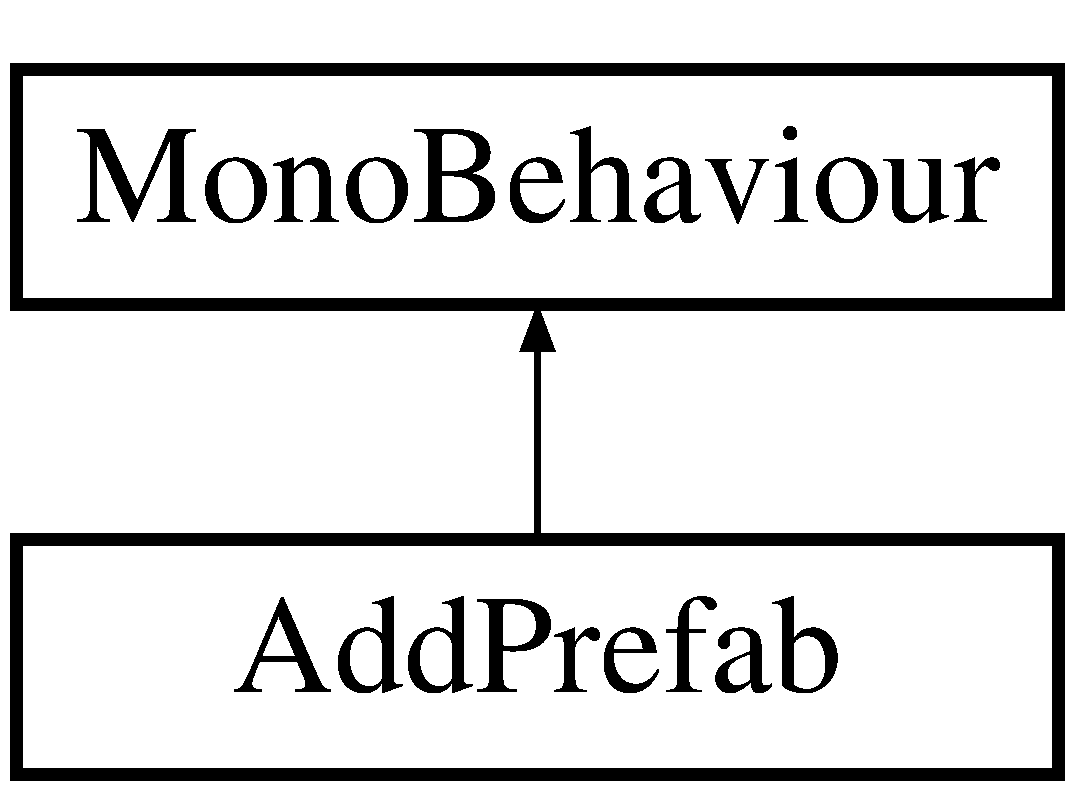
\includegraphics[height=2.000000cm]{class_add_prefab}
\end{center}
\end{figure}
\subsection*{Public Attributes}
\begin{DoxyCompactItemize}
\item 
Game\+Object \hyperlink{class_add_prefab_aee46a2acbc563ebf804e9dfbe3d67a05}{prefab}
\end{DoxyCompactItemize}


\subsection{Detailed Description}
Class for adding prefabs pins. 

\begin{DoxyAuthor}{Author}
Piotr Mścichowski 
\end{DoxyAuthor}
\begin{DoxyDate}{Date}
19.\+11.\+2015 created This script should be attached to prefab game object. It waits for key button A, when it\textquotesingle{}s pressed then prefab is added and destroyed 3s after being created to save memory. 
\end{DoxyDate}


\subsection{Member Data Documentation}
\hypertarget{class_add_prefab_aee46a2acbc563ebf804e9dfbe3d67a05}{}\index{Add\+Prefab@{Add\+Prefab}!prefab@{prefab}}
\index{prefab@{prefab}!Add\+Prefab@{Add\+Prefab}}
\subsubsection[{prefab}]{\setlength{\rightskip}{0pt plus 5cm}Game\+Object Add\+Prefab.\+prefab}\label{class_add_prefab_aee46a2acbc563ebf804e9dfbe3d67a05}


The documentation for this class was generated from the following file\+:\begin{DoxyCompactItemize}
\item 
Assets/\+Scripts/\hyperlink{_add_prefab_8cs}{Add\+Prefab.\+cs}\end{DoxyCompactItemize}

\hypertarget{class_ball}{}\section{Ball Class Reference}
\label{class_ball}\index{Ball@{Ball}}


Basic class describing prior settings and behaviour of ball.  


Inheritance diagram for Ball\+:\begin{figure}[H]
\begin{center}
\leavevmode
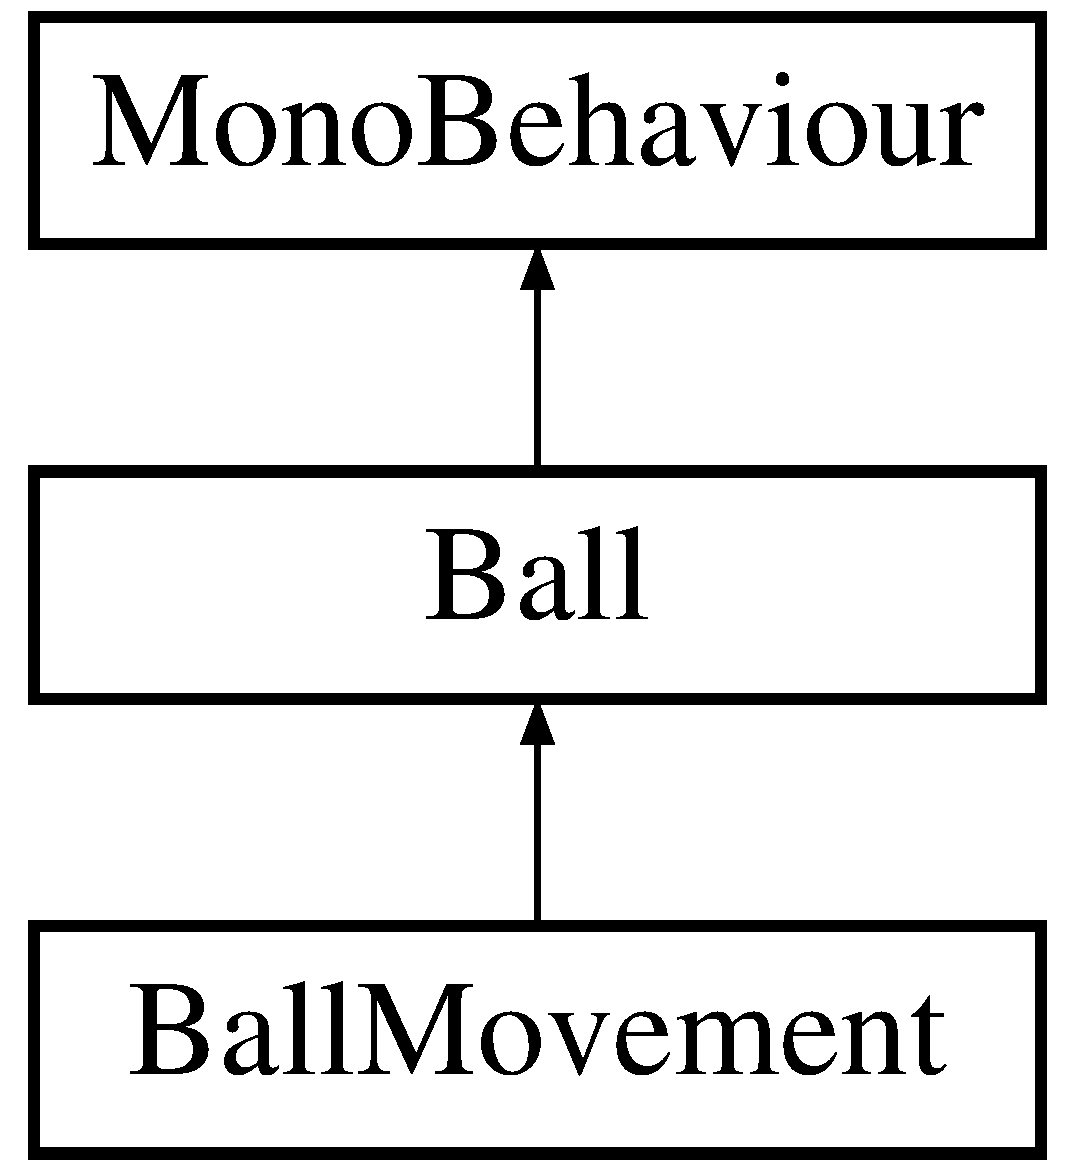
\includegraphics[height=3.000000cm]{class_ball}
\end{center}
\end{figure}
\subsection*{Public Member Functions}
\begin{DoxyCompactItemize}
\item 
virtual void \hyperlink{class_ball_a655a2ac68857807d79d7b32c3dc46b19}{setball\+Speed} (float new\+Speed)
\item 
virtual void \hyperlink{class_ball_ac82387db69cc078a600870dba29a064c}{Start} ()
\begin{DoxyCompactList}\small\item\em Initializes Character\+Controller. \end{DoxyCompactList}\item 
virtual void \hyperlink{class_ball_a237aaf0107c7bf3d7812dc8a9a642593}{Update} ()
\begin{DoxyCompactList}\small\item\em Describes basic control fro keyboard of ball. \end{DoxyCompactList}\end{DoxyCompactItemize}
\subsection*{Public Attributes}
\begin{DoxyCompactItemize}
\item 
Rigidbody \hyperlink{class_ball_ae623e52a072614fd991c767b315c56d7}{controller}
\item 
float \hyperlink{class_ball_a9f152c3ceba4ace75c2c87d73fc40cea}{ball\+Speed} = 0.\+0f
\item 
float \hyperlink{class_ball_a7adb29497e06c56dc9dd0d55ded63aa2}{turn\+Speed} = 90f
\end{DoxyCompactItemize}
\subsection*{Protected Attributes}
\begin{DoxyCompactItemize}
\item 
Vector3 \hyperlink{class_ball_a4fa4815ebae31c377b851144151c9f3d}{move} = Vector3.\+zero
\end{DoxyCompactItemize}


\subsection{Detailed Description}
Basic class describing prior settings and behaviour of ball. 

\begin{DoxyAuthor}{Author}
Piotr Mścichowski 
\end{DoxyAuthor}


\subsection{Member Function Documentation}
\hypertarget{class_ball_a655a2ac68857807d79d7b32c3dc46b19}{}\index{Ball@{Ball}!setball\+Speed@{setball\+Speed}}
\index{setball\+Speed@{setball\+Speed}!Ball@{Ball}}
\subsubsection[{setball\+Speed(float new\+Speed)}]{\setlength{\rightskip}{0pt plus 5cm}virtual void Ball.\+setball\+Speed (
\begin{DoxyParamCaption}
\item[{float}]{new\+Speed}
\end{DoxyParamCaption}
)\hspace{0.3cm}{\ttfamily [virtual]}}\label{class_ball_a655a2ac68857807d79d7b32c3dc46b19}
Sets speed of object \hypertarget{class_ball_ac82387db69cc078a600870dba29a064c}{}\index{Ball@{Ball}!Start@{Start}}
\index{Start@{Start}!Ball@{Ball}}
\subsubsection[{Start()}]{\setlength{\rightskip}{0pt plus 5cm}virtual void Ball.\+Start (
\begin{DoxyParamCaption}
{}
\end{DoxyParamCaption}
)\hspace{0.3cm}{\ttfamily [virtual]}}\label{class_ball_ac82387db69cc078a600870dba29a064c}


Initializes Character\+Controller. 

This method uses Character\+Component to provide basic movement functionality. It is planned to eventually use rigidbody due to force change ability etc. First We want to try movement with character controller but finally probably there will be rigidbody due to force change ability etc.

Reimplemented in \hyperlink{class_ball_movement_a30553c43b5f0edb4ab0b3d1c4b269993}{Ball\+Movement}.

\hypertarget{class_ball_a237aaf0107c7bf3d7812dc8a9a642593}{}\index{Ball@{Ball}!Update@{Update}}
\index{Update@{Update}!Ball@{Ball}}
\subsubsection[{Update()}]{\setlength{\rightskip}{0pt plus 5cm}virtual void Ball.\+Update (
\begin{DoxyParamCaption}
{}
\end{DoxyParamCaption}
)\hspace{0.3cm}{\ttfamily [virtual]}}\label{class_ball_a237aaf0107c7bf3d7812dc8a9a642593}


Describes basic control fro keyboard of ball. 

It uses simple move mode. Movement of object is controlled by arrow keys (up, down, left, right). It also adds possibility to restart game by pressing R. For the begining choosing simple move mode

Reimplemented in \hyperlink{class_ball_movement_adec04489bea52562cc6e1e0048c23bc7}{Ball\+Movement}.



\subsection{Member Data Documentation}
\hypertarget{class_ball_a9f152c3ceba4ace75c2c87d73fc40cea}{}\index{Ball@{Ball}!ball\+Speed@{ball\+Speed}}
\index{ball\+Speed@{ball\+Speed}!Ball@{Ball}}
\subsubsection[{ball\+Speed}]{\setlength{\rightskip}{0pt plus 5cm}float Ball.\+ball\+Speed = 0.\+0f}\label{class_ball_a9f152c3ceba4ace75c2c87d73fc40cea}
\hypertarget{class_ball_ae623e52a072614fd991c767b315c56d7}{}\index{Ball@{Ball}!controller@{controller}}
\index{controller@{controller}!Ball@{Ball}}
\subsubsection[{controller}]{\setlength{\rightskip}{0pt plus 5cm}Rigidbody Ball.\+controller}\label{class_ball_ae623e52a072614fd991c767b315c56d7}
\hypertarget{class_ball_a4fa4815ebae31c377b851144151c9f3d}{}\index{Ball@{Ball}!move@{move}}
\index{move@{move}!Ball@{Ball}}
\subsubsection[{move}]{\setlength{\rightskip}{0pt plus 5cm}Vector3 Ball.\+move = Vector3.\+zero\hspace{0.3cm}{\ttfamily [protected]}}\label{class_ball_a4fa4815ebae31c377b851144151c9f3d}
\hypertarget{class_ball_a7adb29497e06c56dc9dd0d55ded63aa2}{}\index{Ball@{Ball}!turn\+Speed@{turn\+Speed}}
\index{turn\+Speed@{turn\+Speed}!Ball@{Ball}}
\subsubsection[{turn\+Speed}]{\setlength{\rightskip}{0pt plus 5cm}float Ball.\+turn\+Speed = 90f}\label{class_ball_a7adb29497e06c56dc9dd0d55ded63aa2}


The documentation for this class was generated from the following file\+:\begin{DoxyCompactItemize}
\item 
Assets/\+Scripts/\hyperlink{_ball_8cs}{Ball.\+cs}\end{DoxyCompactItemize}

\hypertarget{class_ball_movement}{}\section{Ball\+Movement Class Reference}
\label{class_ball_movement}\index{Ball\+Movement@{Ball\+Movement}}


Derived class for extended controlling ball movement.  


Inheritance diagram for Ball\+Movement\+:\begin{figure}[H]
\begin{center}
\leavevmode
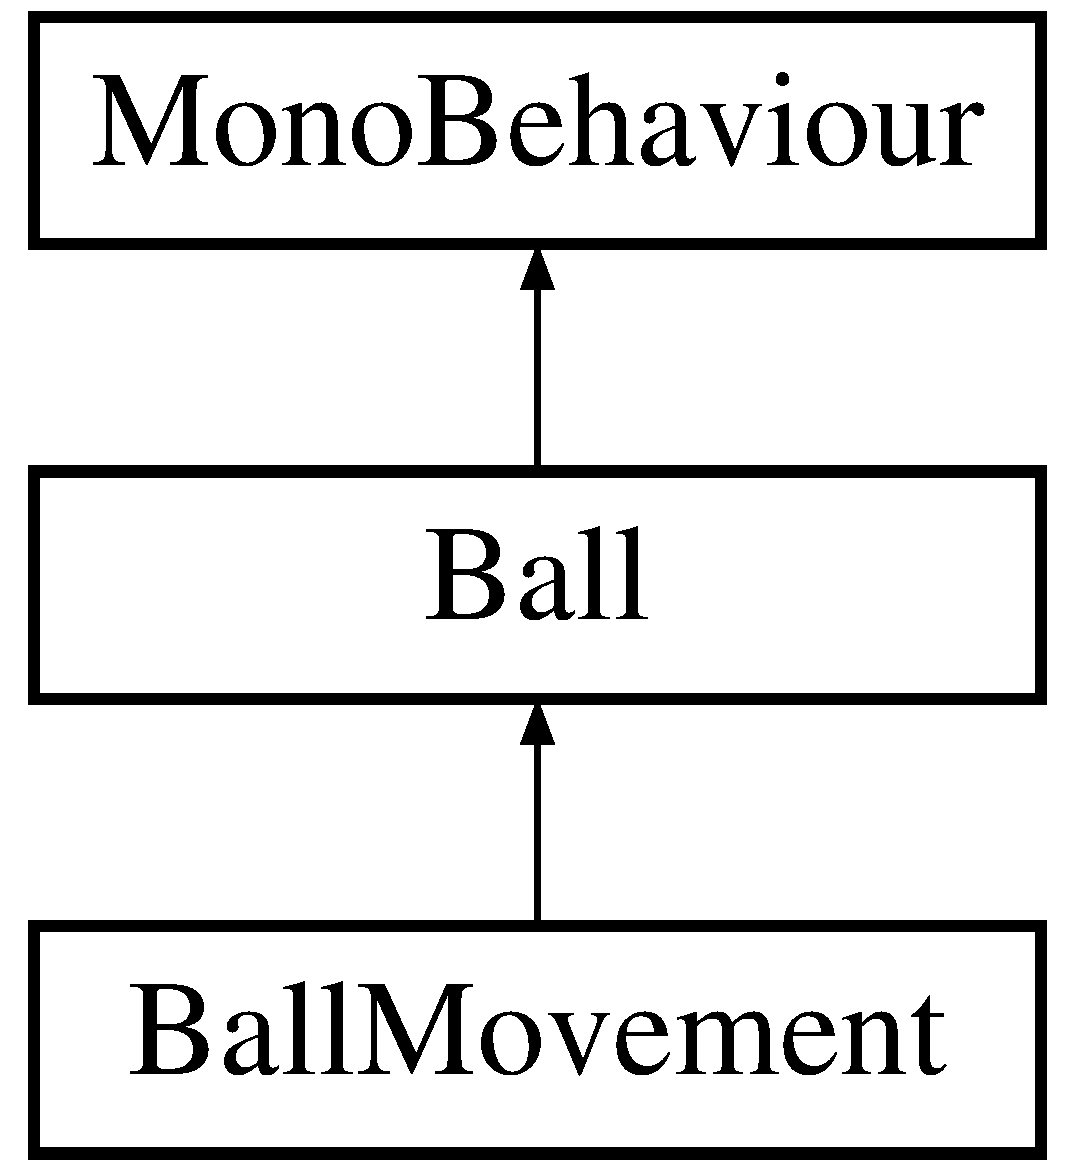
\includegraphics[height=3.000000cm]{class_ball_movement}
\end{center}
\end{figure}
\subsection*{Public Member Functions}
\begin{DoxyCompactItemize}
\item 
override void \hyperlink{class_ball_movement_a30553c43b5f0edb4ab0b3d1c4b269993}{Start} ()
\item 
override void \hyperlink{class_ball_movement_adec04489bea52562cc6e1e0048c23bc7}{Update} ()
\begin{DoxyCompactList}\small\item\em This method is called for every frame. \end{DoxyCompactList}\end{DoxyCompactItemize}
\subsection*{Additional Inherited Members}


\subsection{Detailed Description}
Derived class for extended controlling ball movement. 

\begin{DoxyAuthor}{Author}
Piotr Mścichowski  19.\+11.\+2015 This class enhances ball movement control by adding possibility to control movement by mouse, not only keyboard. 
\end{DoxyAuthor}


\subsection{Member Function Documentation}
\hypertarget{class_ball_movement_a30553c43b5f0edb4ab0b3d1c4b269993}{}\index{Ball\+Movement@{Ball\+Movement}!Start@{Start}}
\index{Start@{Start}!Ball\+Movement@{Ball\+Movement}}
\subsubsection[{Start()}]{\setlength{\rightskip}{0pt plus 5cm}override void Ball\+Movement.\+Start (
\begin{DoxyParamCaption}
{}
\end{DoxyParamCaption}
)\hspace{0.3cm}{\ttfamily [virtual]}}\label{class_ball_movement_a30553c43b5f0edb4ab0b3d1c4b269993}
It simply calls parent method. 

Reimplemented from \hyperlink{class_ball_ac82387db69cc078a600870dba29a064c}{Ball}.

\hypertarget{class_ball_movement_adec04489bea52562cc6e1e0048c23bc7}{}\index{Ball\+Movement@{Ball\+Movement}!Update@{Update}}
\index{Update@{Update}!Ball\+Movement@{Ball\+Movement}}
\subsubsection[{Update()}]{\setlength{\rightskip}{0pt plus 5cm}override void Ball\+Movement.\+Update (
\begin{DoxyParamCaption}
{}
\end{DoxyParamCaption}
)\hspace{0.3cm}{\ttfamily [virtual]}}\label{class_ball_movement_adec04489bea52562cc6e1e0048c23bc7}


This method is called for every frame. 

If left mouse button is pressed, mouse controls direction in which ball aims. When right mouse key goes down, it stores initial mouse position and starting time. When it goes up, final mouse position is stored and time difference is calculated. Calculated values are then applied to ball movement controller. 

Reimplemented from \hyperlink{class_ball_a237aaf0107c7bf3d7812dc8a9a642593}{Ball}.



The documentation for this class was generated from the following file\+:\begin{DoxyCompactItemize}
\item 
Assets/\+Scripts/\hyperlink{_ball_movement_8cs}{Ball\+Movement.\+cs}\end{DoxyCompactItemize}

\hypertarget{class_camera_switch}{}\section{Camera\+Switch Class Reference}
\label{class_camera_switch}\index{Camera\+Switch@{Camera\+Switch}}


Class for switching cameras.  


Inheritance diagram for Camera\+Switch\+:\begin{figure}[H]
\begin{center}
\leavevmode
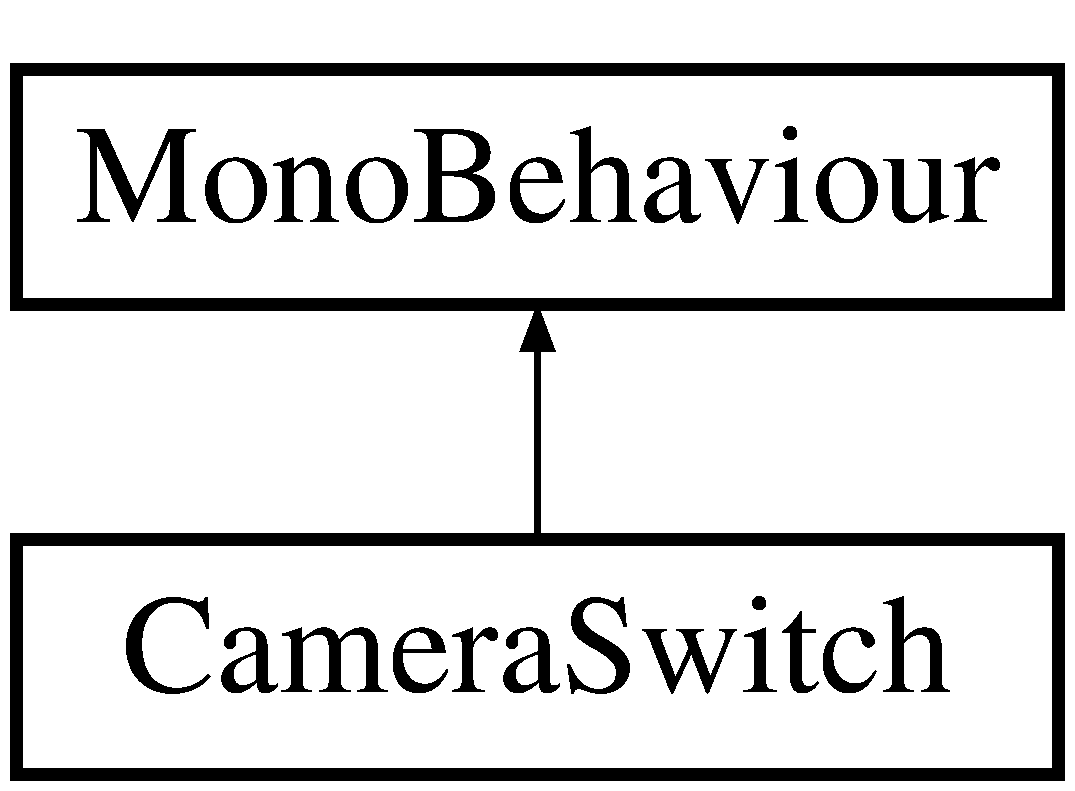
\includegraphics[height=2.000000cm]{class_camera_switch}
\end{center}
\end{figure}
\subsection*{Public Attributes}
\begin{DoxyCompactItemize}
\item 
Camera\mbox{[}$\,$\mbox{]} \hyperlink{class_camera_switch_a4797769d49b74b29a261aa81c820b25d}{cameras}
\begin{DoxyCompactList}\small\item\em Stores all cameras defined in scene. \end{DoxyCompactList}\item 
int \hyperlink{class_camera_switch_a61b4cf53f1fc86e226eefdb6685ab777}{cameras\+Count}
\begin{DoxyCompactList}\small\item\em Stores number of all cameras in scene. \end{DoxyCompactList}\end{DoxyCompactItemize}


\subsection{Detailed Description}
Class for switching cameras. 

\begin{DoxyAuthor}{Author}
Marek Nalepa 
\end{DoxyAuthor}
\begin{DoxyDate}{Date}
29.\+10.\+2015 created
\end{DoxyDate}
This script should be attached to an empty game object. It listens for function key presses. When keys F1-\/\+F3 are pressed, corresponding cameras are activated (so F1 enables first camera, F2 enables second camera and F3 enables third camera). 

\subsection{Member Data Documentation}
\hypertarget{class_camera_switch_a4797769d49b74b29a261aa81c820b25d}{}\index{Camera\+Switch@{Camera\+Switch}!cameras@{cameras}}
\index{cameras@{cameras}!Camera\+Switch@{Camera\+Switch}}
\subsubsection[{cameras}]{\setlength{\rightskip}{0pt plus 5cm}Camera \mbox{[}$\,$\mbox{]} Camera\+Switch.\+cameras}\label{class_camera_switch_a4797769d49b74b29a261aa81c820b25d}


Stores all cameras defined in scene. 

\hypertarget{class_camera_switch_a61b4cf53f1fc86e226eefdb6685ab777}{}\index{Camera\+Switch@{Camera\+Switch}!cameras\+Count@{cameras\+Count}}
\index{cameras\+Count@{cameras\+Count}!Camera\+Switch@{Camera\+Switch}}
\subsubsection[{cameras\+Count}]{\setlength{\rightskip}{0pt plus 5cm}int Camera\+Switch.\+cameras\+Count}\label{class_camera_switch_a61b4cf53f1fc86e226eefdb6685ab777}


Stores number of all cameras in scene. 



The documentation for this class was generated from the following file\+:\begin{DoxyCompactItemize}
\item 
Assets/\+Scripts/\hyperlink{_camera_switch_8cs}{Camera\+Switch.\+cs}\end{DoxyCompactItemize}

\hypertarget{class_circular_pin_move}{}\section{Circular\+Pin\+Move Class Reference}
\label{class_circular_pin_move}\index{Circular\+Pin\+Move@{Circular\+Pin\+Move}}


Script describing circular movement of pin.  


Inheritance diagram for Circular\+Pin\+Move\+:\begin{figure}[H]
\begin{center}
\leavevmode
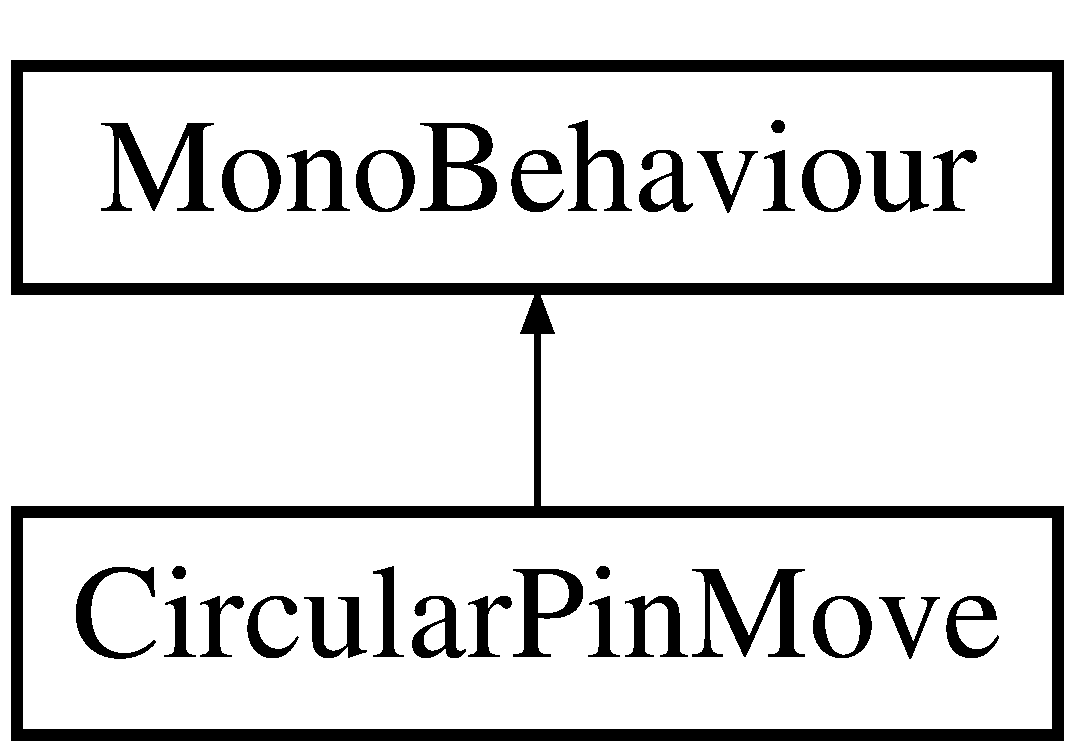
\includegraphics[height=2.000000cm]{class_circular_pin_move}
\end{center}
\end{figure}


\subsection{Detailed Description}
Script describing circular movement of pin. 

\begin{DoxyAuthor}{Author}
Piotr Mścichowski 
\end{DoxyAuthor}
\begin{DoxyDate}{Date}
29.\+10.\+2015 created
\end{DoxyDate}
This script uses X axis values calculated from sinus function and Y axis values calculated from cosinus function. 

The documentation for this class was generated from the following file\+:\begin{DoxyCompactItemize}
\item 
Assets/\+Scripts/\hyperlink{_circular_pin_move_8cs}{Circular\+Pin\+Move.\+cs}\end{DoxyCompactItemize}

\hypertarget{class_color_change}{}\section{Color\+Change Class Reference}
\label{class_color_change}\index{Color\+Change@{Color\+Change}}


Class for controlling object\textquotesingle{}s color change.  


Inheritance diagram for Color\+Change\+:\begin{figure}[H]
\begin{center}
\leavevmode
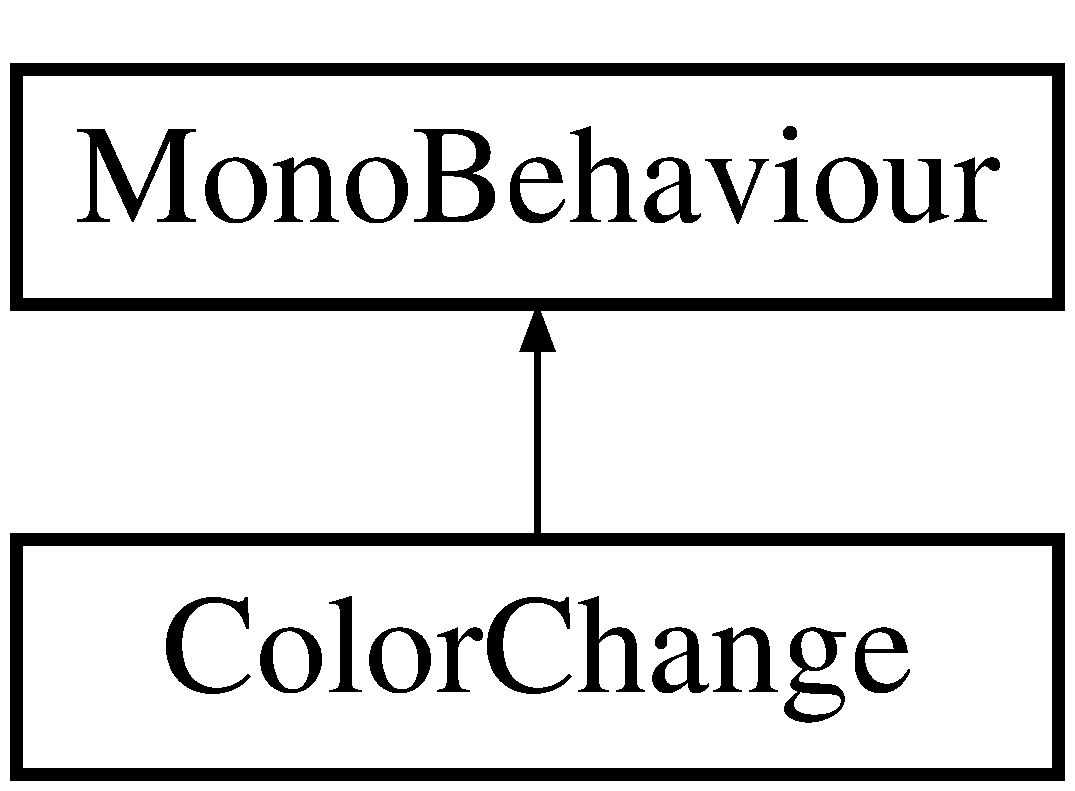
\includegraphics[height=2.000000cm]{class_color_change}
\end{center}
\end{figure}
\subsection*{Public Member Functions}
\begin{DoxyCompactItemize}
\item 
void \hyperlink{class_color_change_a7851038dd8fb7ee037e3572e5ea0820e}{Start} ()
\begin{DoxyCompactList}\small\item\em This method is called on script initialization. \end{DoxyCompactList}\item 
void \hyperlink{class_color_change_adcff0a9a82823d3e0c08ac2aa6dad8c6}{Update} ()
\begin{DoxyCompactList}\small\item\em This method is called for every frame. \end{DoxyCompactList}\end{DoxyCompactItemize}
\subsection*{Public Attributes}
\begin{DoxyCompactItemize}
\item 
Renderer \hyperlink{class_color_change_a325e912ee57c39a0fa9187988dac05de}{ren}
\item 
Color\mbox{[}$\,$\mbox{]} \hyperlink{class_color_change_a82d62c6de3e5c99613d876af2de00627}{possible\+Colors}
\item 
int \hyperlink{class_color_change_a24d6e49ea48325fb5fb722bb80264339}{next\+Color}
\end{DoxyCompactItemize}


\subsection{Detailed Description}
Class for controlling object\textquotesingle{}s color change. 

\begin{DoxyAuthor}{Author}
Marek Nalepa
\end{DoxyAuthor}
This script can be attached to any game object. It provides possibility to change color of object on pressing space key. 

\subsection{Member Function Documentation}
\hypertarget{class_color_change_a7851038dd8fb7ee037e3572e5ea0820e}{}\index{Color\+Change@{Color\+Change}!Start@{Start}}
\index{Start@{Start}!Color\+Change@{Color\+Change}}
\subsubsection[{Start()}]{\setlength{\rightskip}{0pt plus 5cm}void Color\+Change.\+Start (
\begin{DoxyParamCaption}
{}
\end{DoxyParamCaption}
)}\label{class_color_change_a7851038dd8fb7ee037e3572e5ea0820e}


This method is called on script initialization. 

In initialization script aquires game object renderer and stores its reference to future use. Furthermore, the next color index is set to zero. Prevents script from running\hypertarget{class_color_change_adcff0a9a82823d3e0c08ac2aa6dad8c6}{}\index{Color\+Change@{Color\+Change}!Update@{Update}}
\index{Update@{Update}!Color\+Change@{Color\+Change}}
\subsubsection[{Update()}]{\setlength{\rightskip}{0pt plus 5cm}void Color\+Change.\+Update (
\begin{DoxyParamCaption}
{}
\end{DoxyParamCaption}
)}\label{class_color_change_adcff0a9a82823d3e0c08ac2aa6dad8c6}


This method is called for every frame. 

Scripts works when user presses space key. This method checks if space key is pressed down in current frame and assigns next color from array. It also increments next color index. Method does not change colors continuously while user holds space down, only when he first press it. 

\subsection{Member Data Documentation}
\hypertarget{class_color_change_a24d6e49ea48325fb5fb722bb80264339}{}\index{Color\+Change@{Color\+Change}!next\+Color@{next\+Color}}
\index{next\+Color@{next\+Color}!Color\+Change@{Color\+Change}}
\subsubsection[{next\+Color}]{\setlength{\rightskip}{0pt plus 5cm}int Color\+Change.\+next\+Color}\label{class_color_change_a24d6e49ea48325fb5fb722bb80264339}
Index of next color to assign \hypertarget{class_color_change_a82d62c6de3e5c99613d876af2de00627}{}\index{Color\+Change@{Color\+Change}!possible\+Colors@{possible\+Colors}}
\index{possible\+Colors@{possible\+Colors}!Color\+Change@{Color\+Change}}
\subsubsection[{possible\+Colors}]{\setlength{\rightskip}{0pt plus 5cm}Color \mbox{[}$\,$\mbox{]} Color\+Change.\+possible\+Colors}\label{class_color_change_a82d62c6de3e5c99613d876af2de00627}
{\bfseries Initial value\+:}
\begin{DoxyCode}
= \{
        Color.black,
        Color.blue,
        Color.cyan,
        Color.gray,
        Color.green,
        Color.magenta,
        Color.red,
        Color.white,
        Color.yellow
    \}
\end{DoxyCode}
Set of possible colors \hypertarget{class_color_change_a325e912ee57c39a0fa9187988dac05de}{}\index{Color\+Change@{Color\+Change}!ren@{ren}}
\index{ren@{ren}!Color\+Change@{Color\+Change}}
\subsubsection[{ren}]{\setlength{\rightskip}{0pt plus 5cm}Renderer Color\+Change.\+ren}\label{class_color_change_a325e912ee57c39a0fa9187988dac05de}
Game\+Object\textquotesingle{}s Renderer 

The documentation for this class was generated from the following file\+:\begin{DoxyCompactItemize}
\item 
Assets/\+Scripts/\hyperlink{_color_change_8cs}{Color\+Change.\+cs}\end{DoxyCompactItemize}

\hypertarget{class_delete_pin}{}\section{Delete\+Pin Class Reference}
\label{class_delete_pin}\index{Delete\+Pin@{Delete\+Pin}}


Class for deleting pins.  


Inheritance diagram for Delete\+Pin\+:\begin{figure}[H]
\begin{center}
\leavevmode
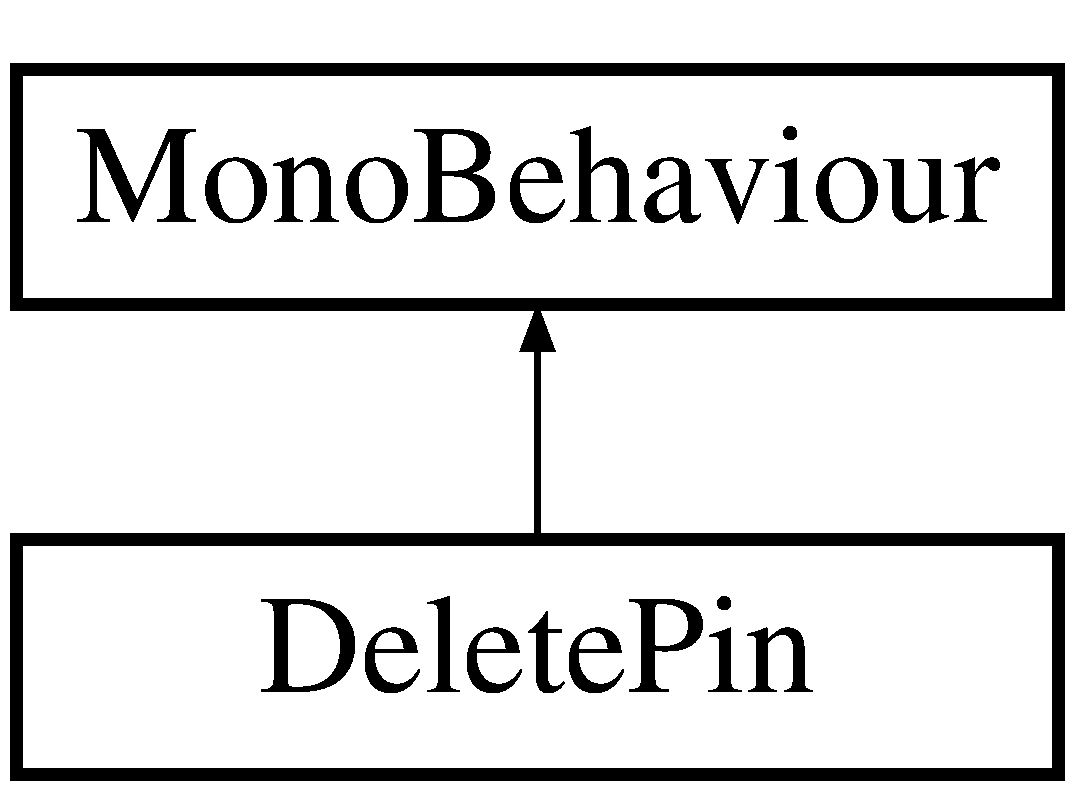
\includegraphics[height=2.000000cm]{class_delete_pin}
\end{center}
\end{figure}


\subsection{Detailed Description}
Class for deleting pins. 

\begin{DoxyAuthor}{Author}
Marek Nalepa 
\end{DoxyAuthor}
\begin{DoxyDate}{Date}
18.\+11.\+2015 created 

20.\+11.\+2015 last updated This script should be attached to floor under track. It checks for collision with game object thath has tag named \textquotesingle{}pin\textquotesingle{}. 
\end{DoxyDate}


The documentation for this class was generated from the following file\+:\begin{DoxyCompactItemize}
\item 
Assets/\+Scripts/\hyperlink{_delete_pin_8cs}{Delete\+Pin.\+cs}\end{DoxyCompactItemize}

\hypertarget{class_ex2_move}{}\section{Ex2\+Move Class Reference}
\label{class_ex2_move}\index{Ex2\+Move@{Ex2\+Move}}


Script describing circular movement of pin with variable speed.  


Inheritance diagram for Ex2\+Move\+:\begin{figure}[H]
\begin{center}
\leavevmode
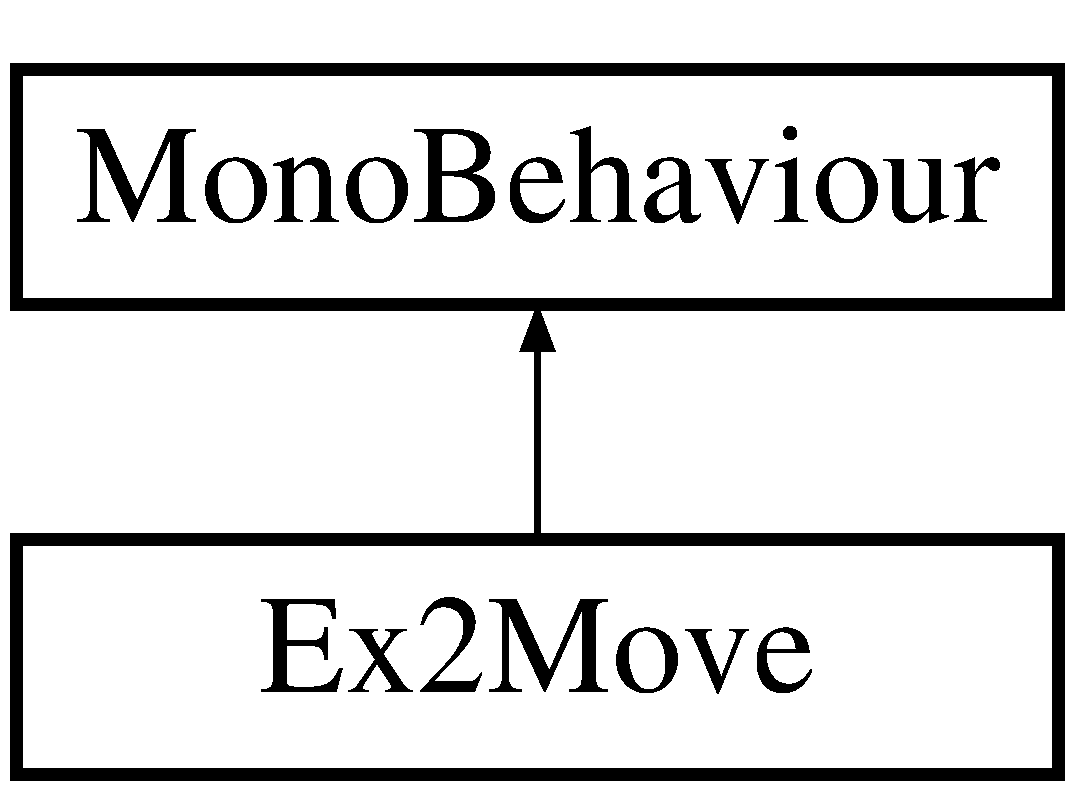
\includegraphics[height=2.000000cm]{class_ex2_move}
\end{center}
\end{figure}


\subsection{Detailed Description}
Script describing circular movement of pin with variable speed. 

\begin{DoxyAuthor}{Author}
Piotr Mścichowski 
\end{DoxyAuthor}
\begin{DoxyDate}{Date}
29.\+10.\+2015 created 

03.\+11.\+2015 last modified
\end{DoxyDate}
This script uses X axis values calculated from sinus function and Y axis values calculated from cosinus function. Additionaly, the movement speed is calculated from time, so it changes during movement. 

The documentation for this class was generated from the following file\+:\begin{DoxyCompactItemize}
\item 
Assets/\+Scripts/\hyperlink{_ex2_move_8cs}{Ex2\+Move.\+cs}\end{DoxyCompactItemize}

\hypertarget{class_explode_script}{}\section{Explode\+Script Class Reference}
\label{class_explode_script}\index{Explode\+Script@{Explode\+Script}}


Class describing pins movement when hitted by ball.  


Inheritance diagram for Explode\+Script\+:\begin{figure}[H]
\begin{center}
\leavevmode
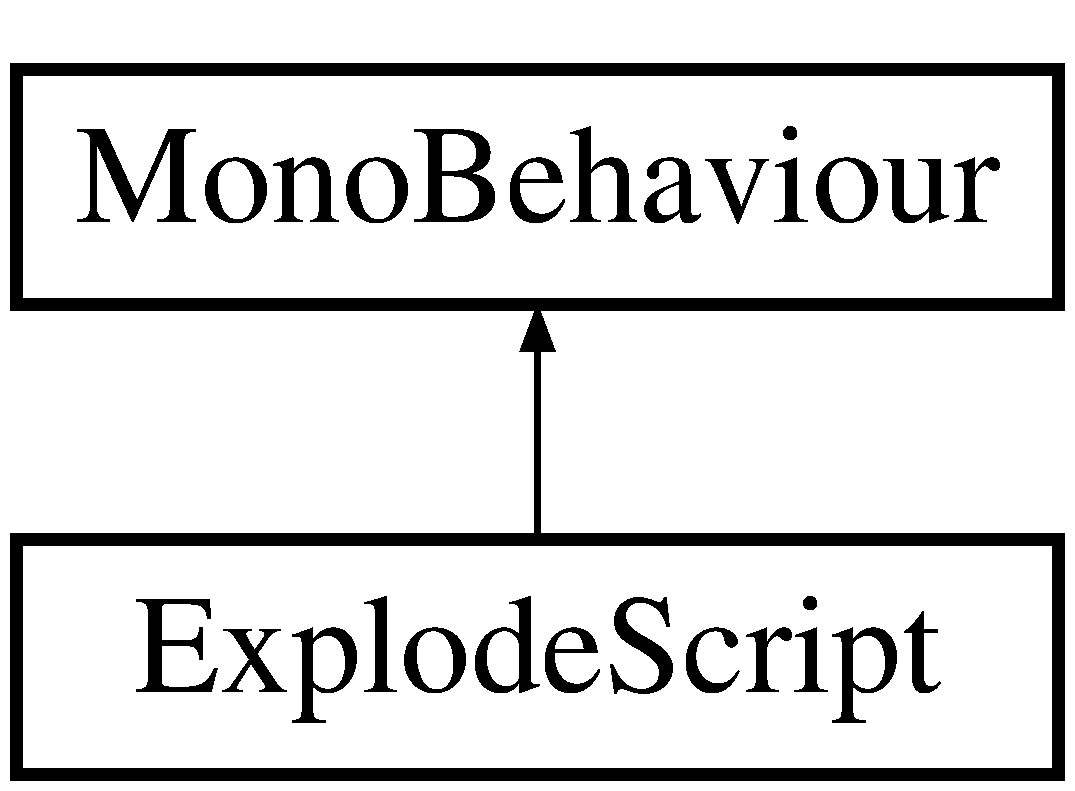
\includegraphics[height=2.000000cm]{class_explode_script}
\end{center}
\end{figure}
\subsection*{Public Attributes}
\begin{DoxyCompactItemize}
\item 
float \hyperlink{class_explode_script_af825236ec0516f880ea50d9bb33c81a1}{force}
\item 
float \hyperlink{class_explode_script_ae208b9d0052339eea0edd81f562b481a}{radius}
\item 
float \hyperlink{class_explode_script_abc4124d039024e334dd726d85c49396e}{up}
\end{DoxyCompactItemize}


\subsection{Detailed Description}
Class describing pins movement when hitted by ball. 

\begin{DoxyAuthor}{Author}
Piotr Mścichowski 
\end{DoxyAuthor}
\begin{DoxyDate}{Date}
19.\+11.\+2015 created 

20.\+11.\+2015 last updated This script should be attached to prefab. It checks for collision with ball(game object with tag called \textquotesingle{}Player\textquotesingle{}). 
\end{DoxyDate}


\subsection{Member Data Documentation}
\hypertarget{class_explode_script_af825236ec0516f880ea50d9bb33c81a1}{}\index{Explode\+Script@{Explode\+Script}!force@{force}}
\index{force@{force}!Explode\+Script@{Explode\+Script}}
\subsubsection[{force}]{\setlength{\rightskip}{0pt plus 5cm}float Explode\+Script.\+force}\label{class_explode_script_af825236ec0516f880ea50d9bb33c81a1}
\hypertarget{class_explode_script_ae208b9d0052339eea0edd81f562b481a}{}\index{Explode\+Script@{Explode\+Script}!radius@{radius}}
\index{radius@{radius}!Explode\+Script@{Explode\+Script}}
\subsubsection[{radius}]{\setlength{\rightskip}{0pt plus 5cm}float Explode\+Script.\+radius}\label{class_explode_script_ae208b9d0052339eea0edd81f562b481a}
\hypertarget{class_explode_script_abc4124d039024e334dd726d85c49396e}{}\index{Explode\+Script@{Explode\+Script}!up@{up}}
\index{up@{up}!Explode\+Script@{Explode\+Script}}
\subsubsection[{up}]{\setlength{\rightskip}{0pt plus 5cm}float Explode\+Script.\+up}\label{class_explode_script_abc4124d039024e334dd726d85c49396e}


The documentation for this class was generated from the following file\+:\begin{DoxyCompactItemize}
\item 
Assets/\+Scripts/\hyperlink{_explode_script_8cs}{Explode\+Script.\+cs}\end{DoxyCompactItemize}

\hypertarget{class_jumping_pins}{}\section{Jumping\+Pins Class Reference}
\label{class_jumping_pins}\index{Jumping\+Pins@{Jumping\+Pins}}


Class describing jump movement of pin.  


Inheritance diagram for Jumping\+Pins\+:\begin{figure}[H]
\begin{center}
\leavevmode
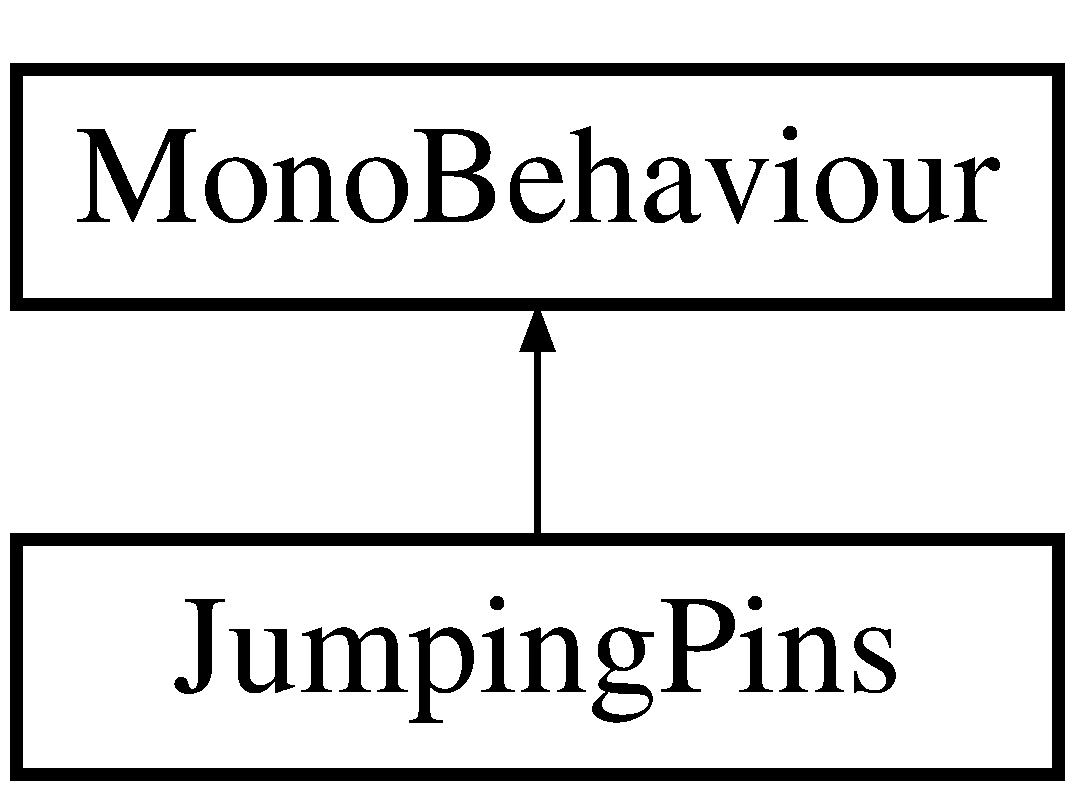
\includegraphics[height=2.000000cm]{class_jumping_pins}
\end{center}
\end{figure}
\subsection*{Public Attributes}
\begin{DoxyCompactItemize}
\item 
float \hyperlink{class_jumping_pins_ae0c8d6f8c73c3efbdaf4e6fbf9a9299d}{radius} = 3.\+0f
\begin{DoxyCompactList}\small\item\em Radius in which explosion should affect. \end{DoxyCompactList}\item 
float \hyperlink{class_jumping_pins_a16bacff923dbd14b883bb6ec3262b78e}{up}
\begin{DoxyCompactList}\small\item\em Vector defining upward movement. \end{DoxyCompactList}\item 
float \hyperlink{class_jumping_pins_af7d195dc1a8351eb4a6f08bd77032e74}{force}
\begin{DoxyCompactList}\small\item\em Force for explosion. \end{DoxyCompactList}\item 
int \hyperlink{class_jumping_pins_a31a3fe87e85993182f3ed08538bf85cf}{max\+Number\+Of\+Collisions}
\begin{DoxyCompactList}\small\item\em Variable definig max number of collision that can occur between objects. \end{DoxyCompactList}\end{DoxyCompactItemize}


\subsection{Detailed Description}
Class describing jump movement of pin. 

\begin{DoxyAuthor}{Author}
Piotr Mścichowski 
\end{DoxyAuthor}
\begin{DoxyDate}{Date}
19.\+11.\+2015 created 

20.\+11.\+2015 last updated This script should be attached to pinf prefab. It checks for collision with track(game object with tag called \textquotesingle{}track\textquotesingle{}). If number of collisions equals set up number, deletes the pin. 
\end{DoxyDate}


\subsection{Member Data Documentation}
\hypertarget{class_jumping_pins_af7d195dc1a8351eb4a6f08bd77032e74}{}\index{Jumping\+Pins@{Jumping\+Pins}!force@{force}}
\index{force@{force}!Jumping\+Pins@{Jumping\+Pins}}
\subsubsection[{force}]{\setlength{\rightskip}{0pt plus 5cm}float Jumping\+Pins.\+force}\label{class_jumping_pins_af7d195dc1a8351eb4a6f08bd77032e74}


Force for explosion. 

\hypertarget{class_jumping_pins_a31a3fe87e85993182f3ed08538bf85cf}{}\index{Jumping\+Pins@{Jumping\+Pins}!max\+Number\+Of\+Collisions@{max\+Number\+Of\+Collisions}}
\index{max\+Number\+Of\+Collisions@{max\+Number\+Of\+Collisions}!Jumping\+Pins@{Jumping\+Pins}}
\subsubsection[{max\+Number\+Of\+Collisions}]{\setlength{\rightskip}{0pt plus 5cm}int Jumping\+Pins.\+max\+Number\+Of\+Collisions}\label{class_jumping_pins_a31a3fe87e85993182f3ed08538bf85cf}


Variable definig max number of collision that can occur between objects. 

\hypertarget{class_jumping_pins_ae0c8d6f8c73c3efbdaf4e6fbf9a9299d}{}\index{Jumping\+Pins@{Jumping\+Pins}!radius@{radius}}
\index{radius@{radius}!Jumping\+Pins@{Jumping\+Pins}}
\subsubsection[{radius}]{\setlength{\rightskip}{0pt plus 5cm}float Jumping\+Pins.\+radius = 3.\+0f}\label{class_jumping_pins_ae0c8d6f8c73c3efbdaf4e6fbf9a9299d}


Radius in which explosion should affect. 

\hypertarget{class_jumping_pins_a16bacff923dbd14b883bb6ec3262b78e}{}\index{Jumping\+Pins@{Jumping\+Pins}!up@{up}}
\index{up@{up}!Jumping\+Pins@{Jumping\+Pins}}
\subsubsection[{up}]{\setlength{\rightskip}{0pt plus 5cm}float Jumping\+Pins.\+up}\label{class_jumping_pins_a16bacff923dbd14b883bb6ec3262b78e}


Vector defining upward movement. 



The documentation for this class was generated from the following file\+:\begin{DoxyCompactItemize}
\item 
Assets/\+Scripts/\hyperlink{_jumping_pins_8cs}{Jumping\+Pins.\+cs}\end{DoxyCompactItemize}

\hypertarget{classlook_at_script}{}\section{look\+At\+Script Class Reference}
\label{classlook_at_script}\index{look\+At\+Script@{look\+At\+Script}}


Camera movement.  


Inheritance diagram for look\+At\+Script\+:\begin{figure}[H]
\begin{center}
\leavevmode
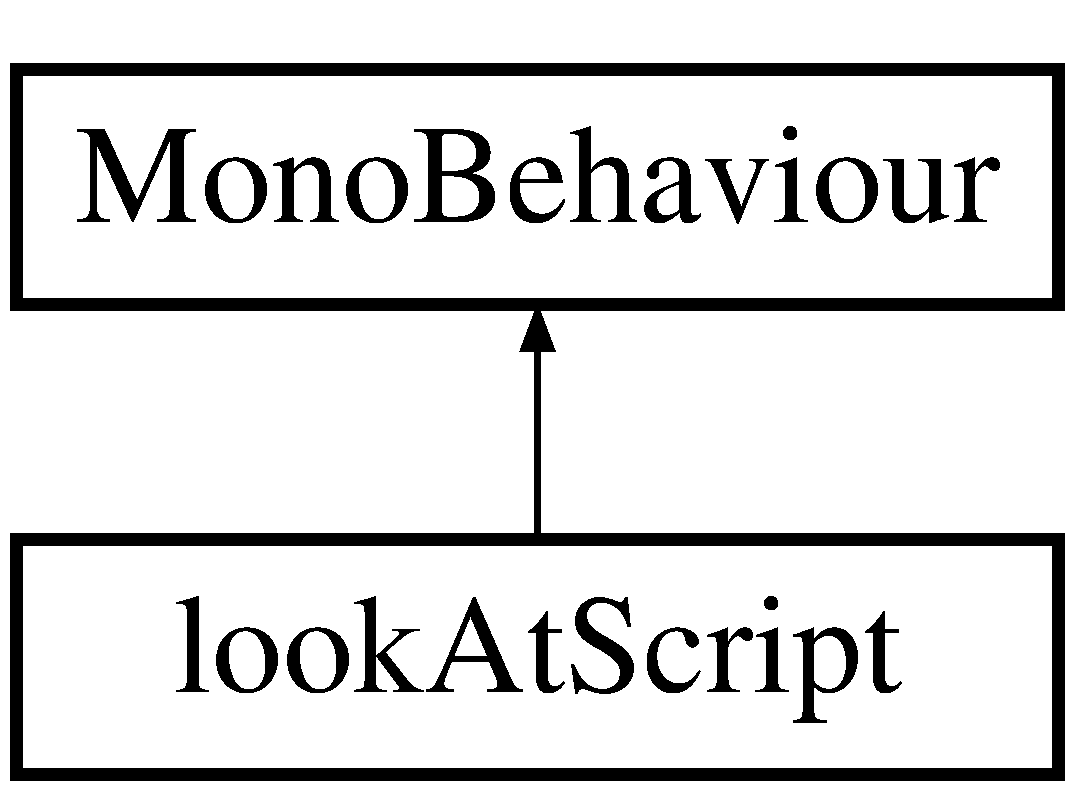
\includegraphics[height=2.000000cm]{classlook_at_script}
\end{center}
\end{figure}
\subsection*{Public Attributes}
\begin{DoxyCompactItemize}
\item 
Transform \hyperlink{classlook_at_script_a3b70e47b1a08454438cd971a9e752a70}{target}
\end{DoxyCompactItemize}


\subsection{Detailed Description}
Camera movement. 

\begin{DoxyAuthor}{Author}
Piotr Mścichowski 
\end{DoxyAuthor}
\begin{DoxyDate}{Date}
19.\+11.\+2015 created 

20.\+11.\+2015 last updated This script should be attached to player, allows camera to follow object 
\end{DoxyDate}


\subsection{Member Data Documentation}
\hypertarget{classlook_at_script_a3b70e47b1a08454438cd971a9e752a70}{}\index{look\+At\+Script@{look\+At\+Script}!target@{target}}
\index{target@{target}!look\+At\+Script@{look\+At\+Script}}
\subsubsection[{target}]{\setlength{\rightskip}{0pt plus 5cm}Transform look\+At\+Script.\+target}\label{classlook_at_script_a3b70e47b1a08454438cd971a9e752a70}


The documentation for this class was generated from the following file\+:\begin{DoxyCompactItemize}
\item 
Assets/\+Scripts/\hyperlink{look_at_script_8cs}{look\+At\+Script.\+cs}\end{DoxyCompactItemize}

\hypertarget{class_object_move}{}\section{Object\+Move Class Reference}
\label{class_object_move}\index{Object\+Move@{Object\+Move}}
Inheritance diagram for Object\+Move\+:\begin{figure}[H]
\begin{center}
\leavevmode
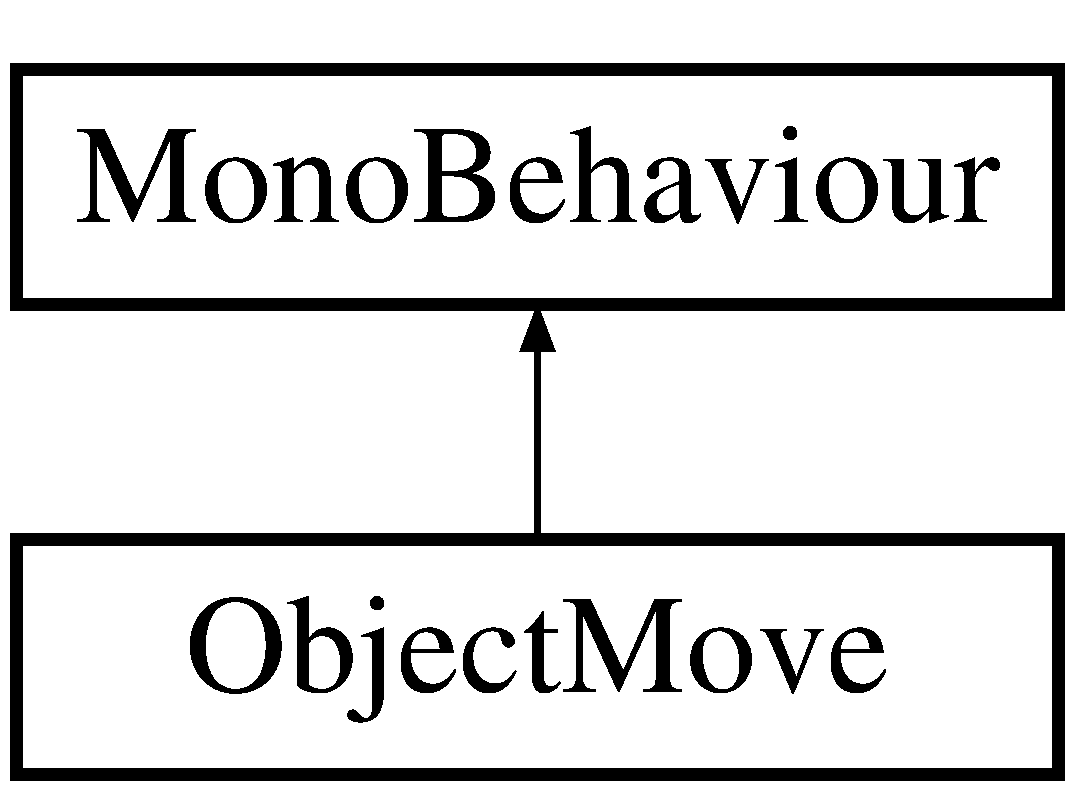
\includegraphics[height=2.000000cm]{class_object_move}
\end{center}
\end{figure}
\subsection*{Public Attributes}
\begin{DoxyCompactItemize}
\item 
Renderer \hyperlink{class_object_move_a7dfb8fd3e835fa77a8f4dfe8092ab026}{ren}
\end{DoxyCompactItemize}


\subsection{Member Data Documentation}
\hypertarget{class_object_move_a7dfb8fd3e835fa77a8f4dfe8092ab026}{}\index{Object\+Move@{Object\+Move}!ren@{ren}}
\index{ren@{ren}!Object\+Move@{Object\+Move}}
\subsubsection[{ren}]{\setlength{\rightskip}{0pt plus 5cm}Renderer Object\+Move.\+ren}\label{class_object_move_a7dfb8fd3e835fa77a8f4dfe8092ab026}


The documentation for this class was generated from the following file\+:\begin{DoxyCompactItemize}
\item 
Assets/\+Scripts/\hyperlink{_object_move_8cs}{Object\+Move.\+cs}\end{DoxyCompactItemize}

\hypertarget{class_pin_fall_down}{}\section{Pin\+Fall\+Down Class Reference}
\label{class_pin_fall_down}\index{Pin\+Fall\+Down@{Pin\+Fall\+Down}}


Class discribing explosion of bowling pins connected with key event.  


Inheritance diagram for Pin\+Fall\+Down\+:\begin{figure}[H]
\begin{center}
\leavevmode
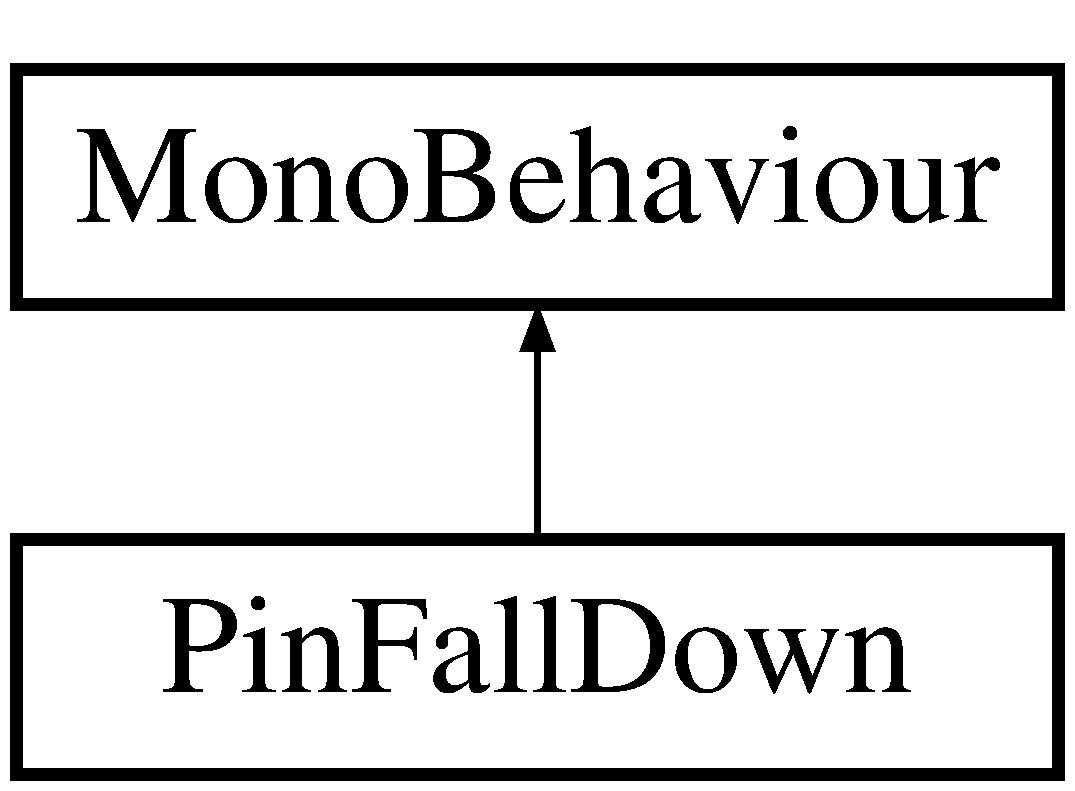
\includegraphics[height=2.000000cm]{class_pin_fall_down}
\end{center}
\end{figure}
\subsection*{Public Attributes}
\begin{DoxyCompactItemize}
\item 
float \hyperlink{class_pin_fall_down_aa89b8c30295e795a3355e45fd4def19e}{radius} = 2.\+0\+F
\begin{DoxyCompactList}\small\item\em Radius of sphere where script takes effect. \end{DoxyCompactList}\item 
float \hyperlink{class_pin_fall_down_a8658bded276508aad0b6297af75b5d56}{power} = 50.\+0\+F
\begin{DoxyCompactList}\small\item\em Force of explosion. \end{DoxyCompactList}\end{DoxyCompactItemize}


\subsection{Detailed Description}
Class discribing explosion of bowling pins connected with key event. 

\begin{DoxyAuthor}{Author}
Piotr Mścichowski 
\end{DoxyAuthor}
\begin{DoxyDate}{Date}
30.\+10.\+2015 created 

04.\+11.\+2015 last edited
\end{DoxyDate}
This script adds explosion force to game object to move it. 

\subsection{Member Data Documentation}
\hypertarget{class_pin_fall_down_a8658bded276508aad0b6297af75b5d56}{}\index{Pin\+Fall\+Down@{Pin\+Fall\+Down}!power@{power}}
\index{power@{power}!Pin\+Fall\+Down@{Pin\+Fall\+Down}}
\subsubsection[{power}]{\setlength{\rightskip}{0pt plus 5cm}float Pin\+Fall\+Down.\+power = 50.\+0\+F}\label{class_pin_fall_down_a8658bded276508aad0b6297af75b5d56}


Force of explosion. 

\hypertarget{class_pin_fall_down_aa89b8c30295e795a3355e45fd4def19e}{}\index{Pin\+Fall\+Down@{Pin\+Fall\+Down}!radius@{radius}}
\index{radius@{radius}!Pin\+Fall\+Down@{Pin\+Fall\+Down}}
\subsubsection[{radius}]{\setlength{\rightskip}{0pt plus 5cm}float Pin\+Fall\+Down.\+radius = 2.\+0\+F}\label{class_pin_fall_down_aa89b8c30295e795a3355e45fd4def19e}


Radius of sphere where script takes effect. 



The documentation for this class was generated from the following file\+:\begin{DoxyCompactItemize}
\item 
Assets/\+Scripts/\hyperlink{_pin_fall_down_8cs}{Pin\+Fall\+Down.\+cs}\end{DoxyCompactItemize}

\hypertarget{class_square_move}{}\section{Square\+Move Class Reference}
\label{class_square_move}\index{Square\+Move@{Square\+Move}}


Script for moving object along square.  


Inheritance diagram for Square\+Move\+:\begin{figure}[H]
\begin{center}
\leavevmode
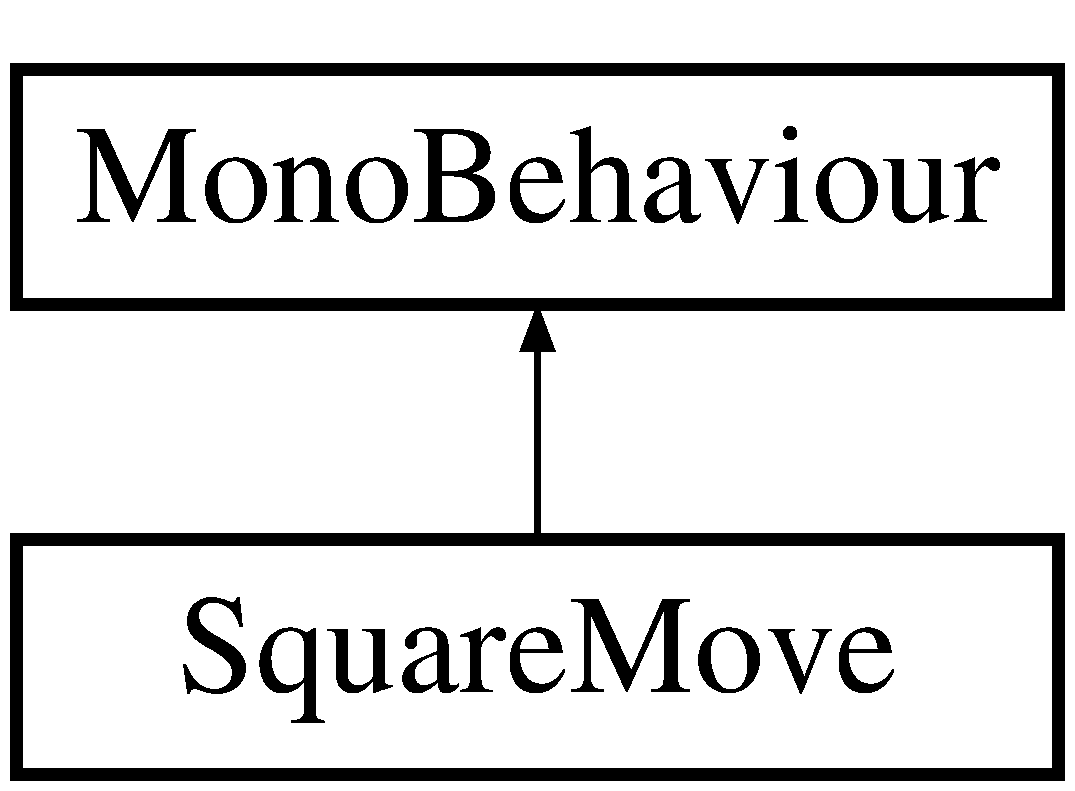
\includegraphics[height=2.000000cm]{class_square_move}
\end{center}
\end{figure}


\subsection{Detailed Description}
Script for moving object along square. 

\begin{DoxyAuthor}{Author}
Marek Nalepa 
\end{DoxyAuthor}
\begin{DoxyDate}{Date}
04.\+11.\+2015 created
\end{DoxyDate}
Square movement can be described by four parts\+: two on one axis (there and back) and two on another. This script runs in 4 different modes, changing them on time basis. Each mode moves object in one direction on one axis. 

The documentation for this class was generated from the following file\+:\begin{DoxyCompactItemize}
\item 
Assets/\+Scripts/\hyperlink{_square_move_8cs}{Square\+Move.\+cs}\end{DoxyCompactItemize}

\hypertarget{classsuper_script}{}\section{super\+Script Class Reference}
\label{classsuper_script}\index{super\+Script@{super\+Script}}
Inheritance diagram for super\+Script\+:\begin{figure}[H]
\begin{center}
\leavevmode
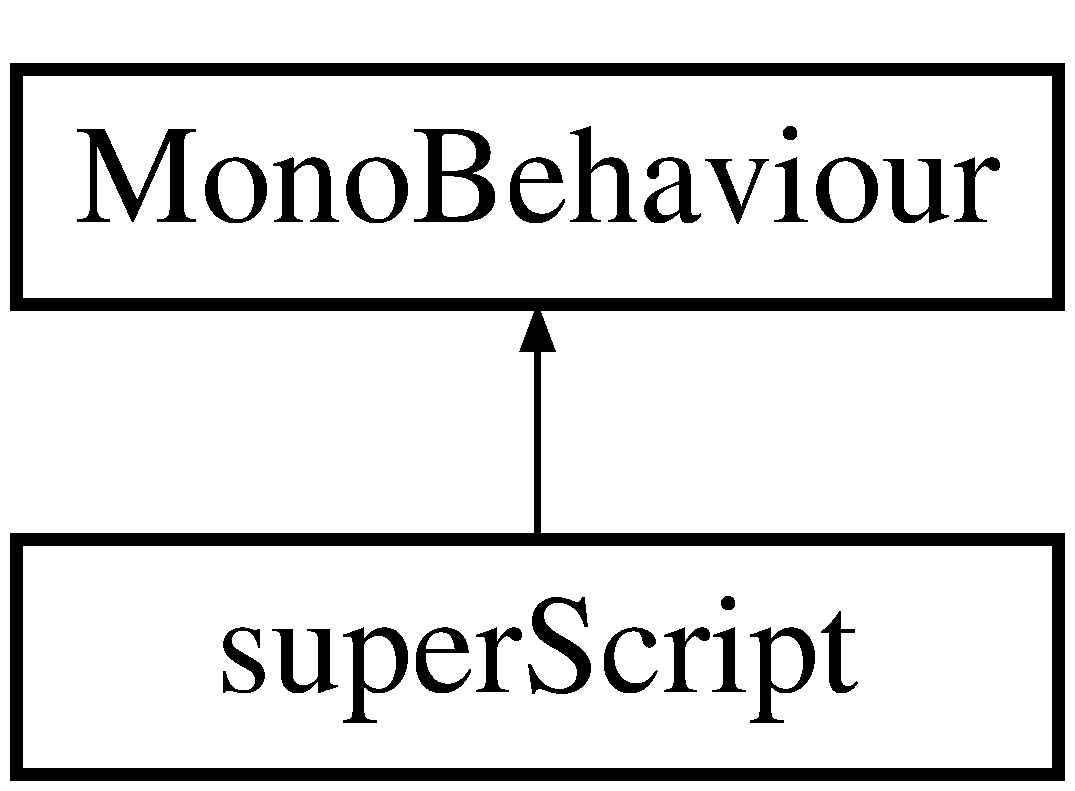
\includegraphics[height=2.000000cm]{classsuper_script}
\end{center}
\end{figure}
\subsection*{Public Attributes}
\begin{DoxyCompactItemize}
\item 
Rigidbody \hyperlink{classsuper_script_a353668fefcd123b158c1c9ee4b27315b}{rb}
\item 
float \hyperlink{classsuper_script_af93edf1af3c4d0ed6666298f8bf7998d}{force} = 1
\end{DoxyCompactItemize}


\subsection{Member Data Documentation}
\hypertarget{classsuper_script_af93edf1af3c4d0ed6666298f8bf7998d}{}\index{super\+Script@{super\+Script}!force@{force}}
\index{force@{force}!super\+Script@{super\+Script}}
\subsubsection[{force}]{\setlength{\rightskip}{0pt plus 5cm}float super\+Script.\+force = 1}\label{classsuper_script_af93edf1af3c4d0ed6666298f8bf7998d}
\hypertarget{classsuper_script_a353668fefcd123b158c1c9ee4b27315b}{}\index{super\+Script@{super\+Script}!rb@{rb}}
\index{rb@{rb}!super\+Script@{super\+Script}}
\subsubsection[{rb}]{\setlength{\rightskip}{0pt plus 5cm}Rigidbody super\+Script.\+rb}\label{classsuper_script_a353668fefcd123b158c1c9ee4b27315b}


The documentation for this class was generated from the following file\+:\begin{DoxyCompactItemize}
\item 
Assets/\+Scripts/\hyperlink{super_script_8cs}{super\+Script.\+cs}\end{DoxyCompactItemize}

\hypertarget{classtest}{}\section{test Class Reference}
\label{classtest}\index{test@{test}}
Inheritance diagram for test\+:\begin{figure}[H]
\begin{center}
\leavevmode
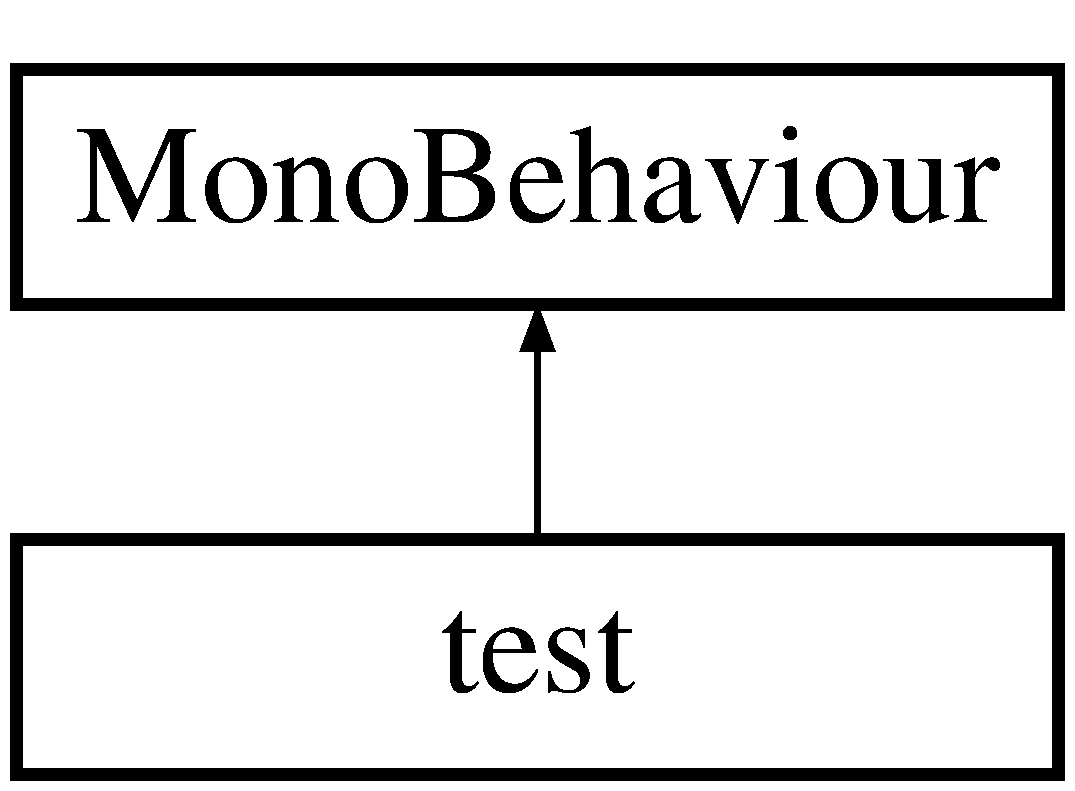
\includegraphics[height=2.000000cm]{classtest}
\end{center}
\end{figure}
\subsection*{Public Attributes}
\begin{DoxyCompactItemize}
\item 
Rigidbody \hyperlink{classtest_ae413e1d589d311bca4f8306e479a5e2d}{body}
\item 
float \hyperlink{classtest_ad02851c5ad217c395ee6c008a652bc93}{force} = 1
\end{DoxyCompactItemize}


\subsection{Member Data Documentation}
\hypertarget{classtest_ae413e1d589d311bca4f8306e479a5e2d}{}\index{test@{test}!body@{body}}
\index{body@{body}!test@{test}}
\subsubsection[{body}]{\setlength{\rightskip}{0pt plus 5cm}Rigidbody test.\+body}\label{classtest_ae413e1d589d311bca4f8306e479a5e2d}
\hypertarget{classtest_ad02851c5ad217c395ee6c008a652bc93}{}\index{test@{test}!force@{force}}
\index{force@{force}!test@{test}}
\subsubsection[{force}]{\setlength{\rightskip}{0pt plus 5cm}float test.\+force = 1}\label{classtest_ad02851c5ad217c395ee6c008a652bc93}


The documentation for this class was generated from the following file\+:\begin{DoxyCompactItemize}
\item 
Assets/\+Scripts/\hyperlink{test_8cs}{test.\+cs}\end{DoxyCompactItemize}

\hypertarget{class_tmp_move}{}\section{Tmp\+Move Class Reference}
\label{class_tmp_move}\index{Tmp\+Move@{Tmp\+Move}}
Inheritance diagram for Tmp\+Move\+:\begin{figure}[H]
\begin{center}
\leavevmode
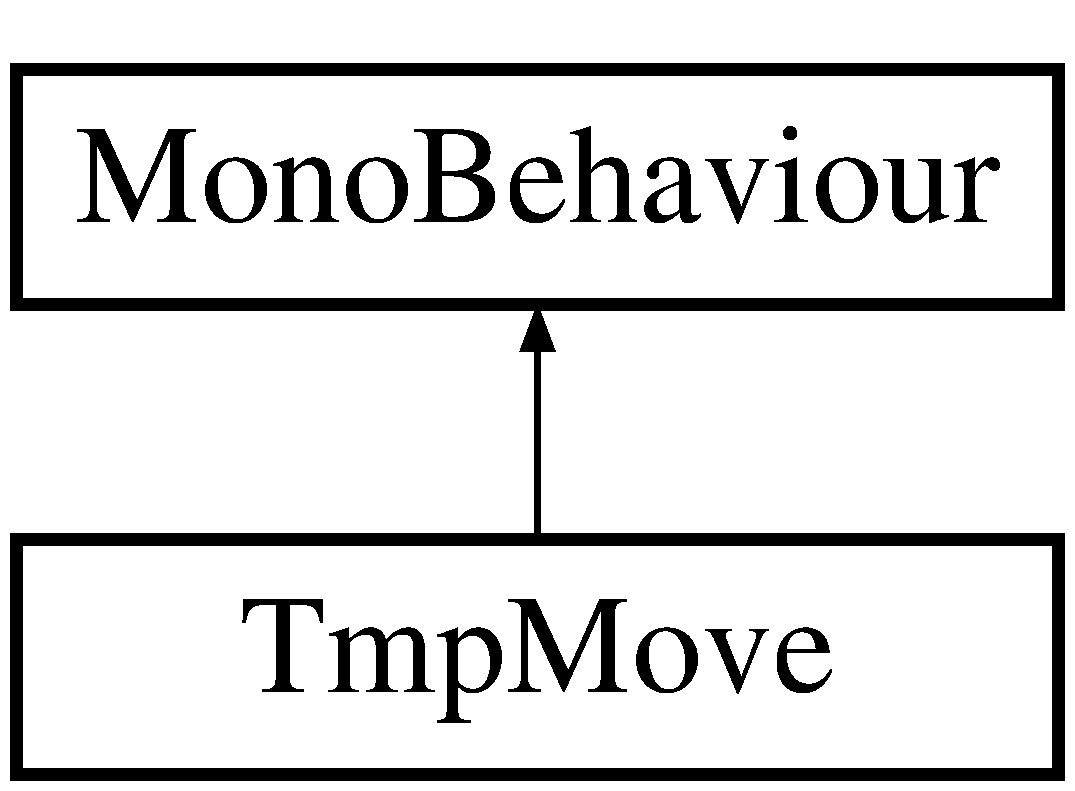
\includegraphics[height=2.000000cm]{class_tmp_move}
\end{center}
\end{figure}
\subsection*{Public Attributes}
\begin{DoxyCompactItemize}
\item 
Rigidbody \hyperlink{class_tmp_move_aa86725b4d9840fc85ccb90522fc72f70}{body}
\item 
bool \hyperlink{class_tmp_move_ace01696c72f650fc1236a8fa61f25bdb}{move\+Left}
\item 
bool \hyperlink{class_tmp_move_a6130ea3b4538fa1761dfc4aeb5cc4ac3}{move\+Right}
\item 
float \hyperlink{class_tmp_move_a2537f998679f53ecc891a26d134e88d2}{radius} = 3.\+0f
\item 
float \hyperlink{class_tmp_move_acd3157eed57aa98545625c0e743d7744}{up} = 100.\+0f
\item 
float \hyperlink{class_tmp_move_a9794fc2a6dbb724a2f2fd136d31b4b56}{force} = 10.\+0f
\end{DoxyCompactItemize}


\subsection{Member Data Documentation}
\hypertarget{class_tmp_move_aa86725b4d9840fc85ccb90522fc72f70}{}\index{Tmp\+Move@{Tmp\+Move}!body@{body}}
\index{body@{body}!Tmp\+Move@{Tmp\+Move}}
\subsubsection[{body}]{\setlength{\rightskip}{0pt plus 5cm}Rigidbody Tmp\+Move.\+body}\label{class_tmp_move_aa86725b4d9840fc85ccb90522fc72f70}
\hypertarget{class_tmp_move_a9794fc2a6dbb724a2f2fd136d31b4b56}{}\index{Tmp\+Move@{Tmp\+Move}!force@{force}}
\index{force@{force}!Tmp\+Move@{Tmp\+Move}}
\subsubsection[{force}]{\setlength{\rightskip}{0pt plus 5cm}float Tmp\+Move.\+force = 10.\+0f}\label{class_tmp_move_a9794fc2a6dbb724a2f2fd136d31b4b56}
\hypertarget{class_tmp_move_ace01696c72f650fc1236a8fa61f25bdb}{}\index{Tmp\+Move@{Tmp\+Move}!move\+Left@{move\+Left}}
\index{move\+Left@{move\+Left}!Tmp\+Move@{Tmp\+Move}}
\subsubsection[{move\+Left}]{\setlength{\rightskip}{0pt plus 5cm}bool Tmp\+Move.\+move\+Left}\label{class_tmp_move_ace01696c72f650fc1236a8fa61f25bdb}
\hypertarget{class_tmp_move_a6130ea3b4538fa1761dfc4aeb5cc4ac3}{}\index{Tmp\+Move@{Tmp\+Move}!move\+Right@{move\+Right}}
\index{move\+Right@{move\+Right}!Tmp\+Move@{Tmp\+Move}}
\subsubsection[{move\+Right}]{\setlength{\rightskip}{0pt plus 5cm}bool Tmp\+Move.\+move\+Right}\label{class_tmp_move_a6130ea3b4538fa1761dfc4aeb5cc4ac3}
\hypertarget{class_tmp_move_a2537f998679f53ecc891a26d134e88d2}{}\index{Tmp\+Move@{Tmp\+Move}!radius@{radius}}
\index{radius@{radius}!Tmp\+Move@{Tmp\+Move}}
\subsubsection[{radius}]{\setlength{\rightskip}{0pt plus 5cm}float Tmp\+Move.\+radius = 3.\+0f}\label{class_tmp_move_a2537f998679f53ecc891a26d134e88d2}
\hypertarget{class_tmp_move_acd3157eed57aa98545625c0e743d7744}{}\index{Tmp\+Move@{Tmp\+Move}!up@{up}}
\index{up@{up}!Tmp\+Move@{Tmp\+Move}}
\subsubsection[{up}]{\setlength{\rightskip}{0pt plus 5cm}float Tmp\+Move.\+up = 100.\+0f}\label{class_tmp_move_acd3157eed57aa98545625c0e743d7744}


The documentation for this class was generated from the following file\+:\begin{DoxyCompactItemize}
\item 
Assets/\+Scripts/\hyperlink{_tmp_move_8cs}{Tmp\+Move.\+cs}\end{DoxyCompactItemize}

\chapter{File Documentation}
\hypertarget{_add_prefab_8cs}{}\section{Assets/\+Scripts/\+Add\+Prefab.cs File Reference}
\label{_add_prefab_8cs}\index{Assets/\+Scripts/\+Add\+Prefab.\+cs@{Assets/\+Scripts/\+Add\+Prefab.\+cs}}
\subsection*{Classes}
\begin{DoxyCompactItemize}
\item 
class \hyperlink{class_add_prefab}{Add\+Prefab}
\begin{DoxyCompactList}\small\item\em Class for adding prefabs pins. \end{DoxyCompactList}\end{DoxyCompactItemize}

\hypertarget{_ball_8cs}{}\section{Assets/\+Scripts/\+Ball.cs File Reference}
\label{_ball_8cs}\index{Assets/\+Scripts/\+Ball.\+cs@{Assets/\+Scripts/\+Ball.\+cs}}
\subsection*{Classes}
\begin{DoxyCompactItemize}
\item 
class \hyperlink{class_ball}{Ball}
\begin{DoxyCompactList}\small\item\em Basic class describing prior settings and behaviour of ball. \end{DoxyCompactList}\end{DoxyCompactItemize}

\hypertarget{_ball_movement_8cs}{}\section{Assets/\+Scripts/\+Ball\+Movement.cs File Reference}
\label{_ball_movement_8cs}\index{Assets/\+Scripts/\+Ball\+Movement.\+cs@{Assets/\+Scripts/\+Ball\+Movement.\+cs}}
\subsection*{Classes}
\begin{DoxyCompactItemize}
\item 
class \hyperlink{class_ball_movement}{Ball\+Movement}
\begin{DoxyCompactList}\small\item\em Derived class for extended controlling ball movement. \end{DoxyCompactList}\end{DoxyCompactItemize}

\hypertarget{_camera_switch_8cs}{}\section{Assets/\+Scripts/\+Camera\+Switch.cs File Reference}
\label{_camera_switch_8cs}\index{Assets/\+Scripts/\+Camera\+Switch.\+cs@{Assets/\+Scripts/\+Camera\+Switch.\+cs}}
\subsection*{Classes}
\begin{DoxyCompactItemize}
\item 
class \hyperlink{class_camera_switch}{Camera\+Switch}
\begin{DoxyCompactList}\small\item\em Class for switching cameras. \end{DoxyCompactList}\end{DoxyCompactItemize}

\hypertarget{_circular_pin_move_8cs}{}\section{Assets/\+Scripts/\+Circular\+Pin\+Move.cs File Reference}
\label{_circular_pin_move_8cs}\index{Assets/\+Scripts/\+Circular\+Pin\+Move.\+cs@{Assets/\+Scripts/\+Circular\+Pin\+Move.\+cs}}
\subsection*{Classes}
\begin{DoxyCompactItemize}
\item 
class \hyperlink{class_circular_pin_move}{Circular\+Pin\+Move}
\begin{DoxyCompactList}\small\item\em Script describing circular movement of pin. \end{DoxyCompactList}\end{DoxyCompactItemize}

\hypertarget{_color_change_8cs}{}\section{Assets/\+Scripts/\+Color\+Change.cs File Reference}
\label{_color_change_8cs}\index{Assets/\+Scripts/\+Color\+Change.\+cs@{Assets/\+Scripts/\+Color\+Change.\+cs}}
\subsection*{Classes}
\begin{DoxyCompactItemize}
\item 
class \hyperlink{class_color_change}{Color\+Change}
\begin{DoxyCompactList}\small\item\em Class for controlling object\textquotesingle{}s color change. \end{DoxyCompactList}\end{DoxyCompactItemize}

\hypertarget{_delete_pin_8cs}{}\section{Assets/\+Scripts/\+Delete\+Pin.cs File Reference}
\label{_delete_pin_8cs}\index{Assets/\+Scripts/\+Delete\+Pin.\+cs@{Assets/\+Scripts/\+Delete\+Pin.\+cs}}
\subsection*{Classes}
\begin{DoxyCompactItemize}
\item 
class \hyperlink{class_delete_pin}{Delete\+Pin}
\begin{DoxyCompactList}\small\item\em Class for deleting pins. \end{DoxyCompactList}\end{DoxyCompactItemize}

\hypertarget{_ex2_move_8cs}{}\section{Assets/\+Scripts/\+Ex2\+Move.cs File Reference}
\label{_ex2_move_8cs}\index{Assets/\+Scripts/\+Ex2\+Move.\+cs@{Assets/\+Scripts/\+Ex2\+Move.\+cs}}
\subsection*{Classes}
\begin{DoxyCompactItemize}
\item 
class \hyperlink{class_ex2_move}{Ex2\+Move}
\begin{DoxyCompactList}\small\item\em Script describing circular movement of pin with variable speed. \end{DoxyCompactList}\end{DoxyCompactItemize}

\hypertarget{_explode_script_8cs}{}\section{Assets/\+Scripts/\+Explode\+Script.cs File Reference}
\label{_explode_script_8cs}\index{Assets/\+Scripts/\+Explode\+Script.\+cs@{Assets/\+Scripts/\+Explode\+Script.\+cs}}
\subsection*{Classes}
\begin{DoxyCompactItemize}
\item 
class \hyperlink{class_explode_script}{Explode\+Script}
\begin{DoxyCompactList}\small\item\em Class describing pins movement when hitted by ball. \end{DoxyCompactList}\end{DoxyCompactItemize}

\hypertarget{_jumping_pins_8cs}{}\section{Assets/\+Scripts/\+Jumping\+Pins.cs File Reference}
\label{_jumping_pins_8cs}\index{Assets/\+Scripts/\+Jumping\+Pins.\+cs@{Assets/\+Scripts/\+Jumping\+Pins.\+cs}}
\subsection*{Classes}
\begin{DoxyCompactItemize}
\item 
class \hyperlink{class_jumping_pins}{Jumping\+Pins}
\begin{DoxyCompactList}\small\item\em Class describing jump movement of pin. \end{DoxyCompactList}\end{DoxyCompactItemize}

\hypertarget{look_at_script_8cs}{}\section{Assets/\+Scripts/look\+At\+Script.cs File Reference}
\label{look_at_script_8cs}\index{Assets/\+Scripts/look\+At\+Script.\+cs@{Assets/\+Scripts/look\+At\+Script.\+cs}}
\subsection*{Classes}
\begin{DoxyCompactItemize}
\item 
class \hyperlink{classlook_at_script}{look\+At\+Script}
\begin{DoxyCompactList}\small\item\em Camera movement. \end{DoxyCompactList}\end{DoxyCompactItemize}

\hypertarget{_object_move_8cs}{}\section{Assets/\+Scripts/\+Object\+Move.cs File Reference}
\label{_object_move_8cs}\index{Assets/\+Scripts/\+Object\+Move.\+cs@{Assets/\+Scripts/\+Object\+Move.\+cs}}
\subsection*{Classes}
\begin{DoxyCompactItemize}
\item 
class \hyperlink{class_object_move}{Object\+Move}
\end{DoxyCompactItemize}

\hypertarget{_pin_fall_down_8cs}{}\section{Assets/\+Scripts/\+Pin\+Fall\+Down.cs File Reference}
\label{_pin_fall_down_8cs}\index{Assets/\+Scripts/\+Pin\+Fall\+Down.\+cs@{Assets/\+Scripts/\+Pin\+Fall\+Down.\+cs}}
\subsection*{Classes}
\begin{DoxyCompactItemize}
\item 
class \hyperlink{class_pin_fall_down}{Pin\+Fall\+Down}
\begin{DoxyCompactList}\small\item\em Class discribing explosion of bowling pins connected with key event. \end{DoxyCompactList}\end{DoxyCompactItemize}

\hypertarget{_pin_movement_task2_8dox}{}\section{Assets/\+Scripts/\+Pin\+Movement\+Task2.dox File Reference}
\label{_pin_movement_task2_8dox}\index{Assets/\+Scripts/\+Pin\+Movement\+Task2.\+dox@{Assets/\+Scripts/\+Pin\+Movement\+Task2.\+dox}}

\hypertarget{_square_move_8cs}{}\section{Assets/\+Scripts/\+Square\+Move.cs File Reference}
\label{_square_move_8cs}\index{Assets/\+Scripts/\+Square\+Move.\+cs@{Assets/\+Scripts/\+Square\+Move.\+cs}}
\subsection*{Classes}
\begin{DoxyCompactItemize}
\item 
class \hyperlink{class_square_move}{Square\+Move}
\begin{DoxyCompactList}\small\item\em Script for moving object along square. \end{DoxyCompactList}\end{DoxyCompactItemize}

\hypertarget{super_script_8cs}{}\section{Assets/\+Scripts/super\+Script.cs File Reference}
\label{super_script_8cs}\index{Assets/\+Scripts/super\+Script.\+cs@{Assets/\+Scripts/super\+Script.\+cs}}
\subsection*{Classes}
\begin{DoxyCompactItemize}
\item 
class \hyperlink{classsuper_script}{super\+Script}
\end{DoxyCompactItemize}

\hypertarget{test_8cs}{}\section{Assets/\+Scripts/test.cs File Reference}
\label{test_8cs}\index{Assets/\+Scripts/test.\+cs@{Assets/\+Scripts/test.\+cs}}
\subsection*{Classes}
\begin{DoxyCompactItemize}
\item 
class \hyperlink{classtest}{test}
\end{DoxyCompactItemize}

\hypertarget{_tmp_move_8cs}{}\section{Assets/\+Scripts/\+Tmp\+Move.cs File Reference}
\label{_tmp_move_8cs}\index{Assets/\+Scripts/\+Tmp\+Move.\+cs@{Assets/\+Scripts/\+Tmp\+Move.\+cs}}
\subsection*{Classes}
\begin{DoxyCompactItemize}
\item 
class \hyperlink{class_tmp_move}{Tmp\+Move}
\end{DoxyCompactItemize}

%--- End generated contents ---

% Index
\backmatter
\newpage
\phantomsection
\clearemptydoublepage
\addcontentsline{toc}{chapter}{Index}
\printindex

\end{document}
